% Welcome! This is the unofficial Umeå University template.
% IMPORTANT: 
% This work, "Umeå University Unofficial Beamer Theme", is a derivative
% of "University of Udine Unofficial Beamer Theme" by Marco Basaldella, University of Udine, CC 4.0 BY. 
% (https://www.overleaf.com/latex/templates/university-of-udine-unofficial-beamer-theme/zndkgxrjsdzt) 
% "Umeå University Unofficial Beamer Theme" is licensed under CC 4.0 by Jesper Erixon.

% See README.md for more full information about this template .

% Note that [usenames,dvipsnames] is MANDATORY due to compatibility
% issues between tikz and xcolor packages.

\documentclass[usenames,dvipsnames]{beamer}
%%%%
\newcommand{\mainfolder}{.}
\newcommand{\writeup}{.}
\newcommand{\basics}{./basics}
\newcommand{\epstopdfimages}{./eps_to_pdf/}
\newcommand{\presentations}{\writeup}
\newcommand{\runfolder}{\presentations}
\newcommand{\runsections}{\runfolder/sections}
\newcommand{\images}{\runfolder/graphics/}
%=====================================================
% NEWCOMMANDS
%=====================================================
\usepackage{mathtools}
\usepackage[utf8]{inputenc}
\usepackage{verbatim}
%\usepackage[english,french]{babel}
\usepackage[english]{babel}
\usepackage{lmodern}
\usepackage{latexsym}
\usepackage[normalem]{ulem}
\renewcommand{\ULdepth}{3pt}

\usepackage{amsmath,amsthm,amsfonts,amssymb,empheq,relsize,alltt}
\usepackage{xparse}
%\usepackage{algorithm}
%\usepackage{algpseudocode}
\usepackage{algorithm2e}
\usepackage{./basics/bbdd/bbdd}
\usepackage{bbm}
\usepackage[singlelinecheck=0,font={sf,small},labelfont=bf]{caption, subfig}
\captionsetup[subfigure]{subrefformat=simple,labelformat=simple,listofformat=subsimple,justification=raggedright}
\usepackage{cancel}
\usepackage{tikz}

\usepackage[noabbrev]{cleveref}
\let\chyperref\cref % Save the orginal command under a new name
\renewcommand{\cref}[1]{\hyperlink{#1}{\chyperref{#1}}} % Redefine the \cref command and explictely add the hyperlink. 
%\usepackage[T1]{fontenc}
\usepackage{media9}
\usepackage{multimedia}
\usepackage{animate}
\usepackage{stmaryrd}
%\usepackage{minted}

\newenvironment{questions}{\begin{list}{\arabic{nquestion}.}{\usecounter{nquestion}\setlength{\itemindent}{-0.5pt}\setlength{\listparindent}{250pt}}}{\unskip\end{list}}
%
\newcommand{\myparagraph}[1]{\subsubsection*{#1}}
% BEAMER
\newcommand{\ptl}[2]{{\large \textcolor{#2}{\textbf{#1}}}}
\newcommand{\cit}[1]{{\tiny \textbf{#1}}}
% TEXTBLOCK
\newcommand{\txb}[4]{
\begin{textblock}{#1}(#2,#3)
	#4
\end{textblock}
}
\newcommand{\blk}[2]{
\begin{block}{#1}
	#2
\end{block}
}
\newcommand{\eblk}[2]{
\begin{exampleblock}{#1}
	#2
\end{exampleblock}
}
\newcommand{\ablk}[2]{
\begin{alertblock}{#1}
	#2
\end{alertblock}
}

\newcommand{\frm}[2]{
\begin{frame}{#1}
	#2
\end{frame}
}
\newcommand{\itmz}[1]{
\begin{itemize}
	#1
\end{itemize}
}
% INCLUDE GRAPHICS WIDTH
\newcommand{\igwf}[2]{
\includegraphics[keepaspectratio,width=#2]{#1}
}
% INCLUDE GRAPHICS HEIGHT
\newcommand{\ighf}[2]{
	\includegraphics[keepaspectratio,height=#2]{#1}
}
% SUBFIGURE
\newcommand{\subf}[2]{
\subfloat[#2]{#1\label{fig:#1}}
}
% SUBFIGURE WIDTH
\newcommand{\subfw}[3]{
	\subfloat[#3]{\igwf{#1}{#2}\label{fig:#1}}
}
% SUBFIGURE HEIGHT
\newcommand{\subfh}[3]{
	\subfloat[#3]{\ighf{#1}{#2}\label{fig:#1}}
}
% BEGIN FIGURE
\newcommand{\bfc}[3]{
\begin{figure}[ht!]
	\centering
	#1
	\caption{#2\label{fig:#3}}
\end{figure}
}
% BEGIN WRAPPED FIGURE
\usepackage{wrapfig}
\usepackage{capt-of}

\DeclareDocumentCommand{\bwfc}{ O{} O{} O{} O{l} O{20mm}}{
	\begin{wrapfigure}{#4}{#5}
		\begin{center}
			#1
			\captionof{figure}{#2}\label{fig:#3}
		\end{center}
\end{wrapfigure}
}

% EQUATION
\newcommand{\beq}[2]{
\begin{equation}
	#1
	\label{eq:#2}
\end{equation}
}
\DeclareDocumentCommand{\beqo}{ O{} O{} O{} }{
	\begin{equation}
	#1
	\label#3{eq:#2}
	\end{equation}
}
\DeclareDocumentCommand{\beqh}{ O{} O{} O{}  O{} }{
	\begin{equation}
	#1
	\hypertarget#3{#4}{\label#3{eq:#2}}
	\end{equation}
}


\DeclareDocumentCommand{\bsys}{ O{} O{} O{} }{
	\begin{empheq}[left=#1\empheqlbrace]{align}
	#2
	\label{eq:#3}
	\end{empheq}
}

\DeclareDocumentCommand{\bmat}{ O{} O{}  }{
	  \begin{bmatrix}
	  	\begin{array}{#2}
		#1
	\end{array}
	\end{bmatrix}
}
\DeclareDocumentCommand{\barr}{ O{} }{
	\begin{array}{c|c}
		#1
	\end{array}
}
%\usepackage{keyval}
%\makeatletter
%\define@key{janbertdims}{l}{\def\janbert@l{#1}}
%\define@key{janbertdims}{w}{\def\janbert@w{#1}}
%\define@key{janbertdims}{h}{\def\janbert@h{#1}}
%% initialize; change here to your preferred values
%\setkeys{janbertdims}{
%	l=1,        
%	w=1,    
%	h=1,
%}
%
%\newcommand\dimsEN[1][]{%
%	\begingroup
%	\setkeys{janbertdims}{#1}% the current values
%	The dimensions ($\mathrm{L} \times \mathrm{W} \times \mathrm{H}$)
%	of the room are
%	$\janbert@l \times \janbert@w \times \janbert@h$%
%	\endgroup
%}
%\makeatother
%
%	\dimsEN
%	
%	\dimsEN[h=3]
%	
%	\dimsEN[h=4,w=2]
%	
%	\dimsEN[w=3,l=5,h=2]
% GGD
\newcommand{\gggd}{$\frac{\text{G}}{\text{G}_\text{max}}-\gamma-\text{D}$ curves }
% KKNPP
\newcommand{\kka}[1][Nuclear Power Plant]{Kashiwazaki-Kariwa #1 }
% NCO
\newcommand{\NCO}{ \textit{Niigata-Ken Ch\={u}etsu-Oki} }
% TEPCO
\newcommand{\TEPCO}{ \textit{Tokyo Electric Power Company} }
% VS/VP/VS30
\newcommand{\vsth}{ V$_\text{S,30}$ }
\newcommand{\vs}{$V_{S}$ }
\newcommand{\vp}{$V_{P}$ }

\newcommand{\N}{\mathbb{N}}
\newcommand{\Z}{\mathbb{Z}}
%\newcommand{\C}{\mathbb{C}}
\DeclareDocumentCommand{\opercal}{O{}O{}O{}}{\ensuremath{\mathcal{#1}_{#2}^{#3}}}
\DeclareDocumentCommand{\operbb}{O{}O{}O{}}{\ensuremath{\mathbb{#1}_{#2}^{#3}}}
% VECTOR
\newcommand{\vct}[3]{\ensuremath{\boldsymbol{\underline{#1}}_{#2}^{#3} }}
\DeclareDocumentCommand{\ebv}{ O{} O{} O{} }{\vct{e}{#1}{#2}#3}
\DeclareDocumentCommand{\Phibv}{ O{} O{} O{} }{\vct{\Phi}{#1}{#2}#3}
\DeclareDocumentCommand{\ibv}{ O{} O{} O{} }{\vct{i}{#1}{#2}#3}

\DeclareDocumentCommand{\ione}{ O{} O{} }{\vct{i}{1}{#1}#2}
\DeclareDocumentCommand{\itwo}{ O{} O{} }{\vct{i}{2}{#1}#2}
\DeclareDocumentCommand{\ithree}{ O{} O{} }{\vct{i}{3}{#1}#2}
\DeclareDocumentCommand{\ix}{ O{} O{} }{\vct{i}{x}{#1}#2}
\DeclareDocumentCommand{\iy}{ O{} O{} }{\vct{i}{y}{#1}#2}

\DeclareDocumentCommand{\ir}{ O{} O{} O{} }{\vct{i}{r_{#1}}{#2}#3}
\DeclareDocumentCommand{\ith}{ O{} O{} O{} }{\vct{i}{\theta_{#1}}{#2}#3}
\DeclareDocumentCommand{\iz}{ O{} O{} O{} }{\vct{i}{z_{#1}}{#2}#3}
% beams
\DeclareDocumentCommand{\eXone}{ O{} }{\ebv[\chi_1]#1}
\DeclareDocumentCommand{\eXtwo}{ O{} }{\ebv[\chi_2]#1}
\DeclareDocumentCommand{\pG}{O{G}}{\pv[#1]}
\DeclareDocumentCommand{\pGp}{O{G} O{\textquotesingle}}{\pv[#1][#2]}
\DeclareDocumentCommand{\psigma}{O{\Sigma}}{\pv[#1]}
\DeclareDocumentCommand{\xG}{O{G}}{\xv[#1]}
\DeclareDocumentCommand{\xGp}{O{G} O{\textquotesingle}}{\xv[#1][#2]}
\DeclareDocumentCommand{\xsigma}{O{\Sigma}}{\xv[#1]}
\DeclareDocumentCommand{\uG}{O{G}}{\uv[#1]}
\DeclareDocumentCommand{\uGp}{O{G} O{\textquotesingle}}{\uv[#1][#2]}
\DeclareDocumentCommand{\uGe}{O{Ge} O{}}{u_{#1}#2}
\DeclareDocumentCommand{\uGep}{O{Ge} O{\textquotesingle}}{u_{#1}^{#2}}
\DeclareDocumentCommand{\uGepp}{O{Ge} O{\textquotesingle\textquotesingle}}{u_{#1}^{#2}}

\DeclareDocumentCommand{\usigma}{O{\Sigma}}{\uv[#1]}
\DeclareDocumentCommand{\uGsigma}{O{G\Sigma}}{\uv[#1]}
\DeclareDocumentCommand{\uGsigmap}{O{G\Sigma} O{\textquotesingle}}{\uv[#1][#2]}
\DeclareDocumentCommand{\uGsigmapp}{O{G\Sigma} O{\textquotesingle\textquotesingle}}{\uv[#1][#2]}

\DeclareDocumentCommand{\uGperp}{O{G\vdash}}{\uv[#1]}
\DeclareDocumentCommand{\uGperpp}{O{G\vdash} O{\textquotesingle}}{\uv[#1][#2]}
\DeclareDocumentCommand{\uGperppp}{O{G\vdash} O{\textquotesingle\textquotesingle}}{\uv[#1][#2]}

\DeclareDocumentCommand{\thetam}{ O{} O{} O{} }{\tens{\theta}{#1}{\wedge}#3}
\DeclareDocumentCommand{\thetav}{ O{} O{} O{} }{\vct{\theta}{#1}{}#3}
\DeclareDocumentCommand{\thetavp}{ O{} O{} }{\vct{\theta}{#1}{\textquotesingle}#2}
\DeclareDocumentCommand{\thsigmap}{ O{} }{\vct{\theta}{\Sigma}{\textquotesingle}#1}
\DeclareDocumentCommand{\thsigmapp}{ O{} }{\vct{\theta}{\Sigma}{\textquotesingle\textquotesingle}#1}
\DeclareDocumentCommand{\thsigma}{ O{\Sigma} O{} O{} }{\vct{\theta}{#1}{#2}#3}
\DeclareDocumentCommand{\thetae}{ O{e} O{} }{\theta_{#1}#2}
\DeclareDocumentCommand{\thetaep}{ O{e} O{\textquotesingle} }{\theta_{#1}^{#2}}
\DeclareDocumentCommand{\thetavperp}{ O{\vdash} O{} }{\vct{\theta}{\vdash}{#2}}
\DeclareDocumentCommand{\dduGv}{ O{} O{} O{} }{\vct{\ddot{u}}{G}{#2}#3}
\DeclareDocumentCommand{\dduGsigma}{ O{} O{} O{} }{\vct{\ddot{u}}{G\Sigma}{#2}#3}
\DeclareDocumentCommand{\ddthetav}{ O{} O{} O{} }{\vct{\ddot{\theta}}{#1}{#2}#3}
\DeclareDocumentCommand{\ddthetae}{}{\ensuremath{\ddot{\theta}_e}}
\DeclareDocumentCommand{\pthp}{ O{} }{\ensuremath{\pdp{\theta_{#1}}} }
\DeclareDocumentCommand{\stressref}{O{ref}}{\ensuremath{\stress \phantom{}_{\text{#1}}}}

\DeclareDocumentCommand{\hv}{ O{} O{} O{} }{\vct{h}{#1}{#2}#3}
\DeclareDocumentCommand{\ov}{ O{} O{} O{} }{\vct{o}{#1}{#2}#3}
\DeclareDocumentCommand{\yv}{ O{} O{} O{} }{\vct{y}{#1}{#2}#3}
\DeclareDocumentCommand{\pv}{ O{} O{} O{} }{\vct{p}{#1}{#2}#3}
\DeclareDocumentCommand{\Xv}{ O{} O{} O{} }{\vct{X}{#1}{#2}#3}
\DeclareDocumentCommand{\xv}{ O{} O{} O{} }{\vct{x}{#1}{#2}#3}
\DeclareDocumentCommand{\xgv}{ O{} O{} O{} }{\vct{x}{g}{#1}#2}
\DeclareDocumentCommand{\ddxgv}{ O{} O{} O{} }{\vct{\ddot{x}}{g}{#1}#2}
\DeclareDocumentCommand{\tv}{ O{} O{} O{} }{\vct{t}{#1}{#2}#3}
\DeclareDocumentCommand{\fv}{ O{} O{} O{} }{\vct{f}{#1}{#2}#3}
\DeclareDocumentCommand{\Ft}{ O{} O{} O{} }{\tens{F}{#1}{#2}#3}
\DeclareDocumentCommand{\cv}{ O{} O{} O{} }{\vct{c}{#1}{#2}#3}
\DeclareDocumentCommand{\Ct}{ O{} O{} O{} }{\tens{C}{#1}{#2}#3}
\DeclareDocumentCommand{\dv}{ O{} O{} O{} }{\vct{d}{#1}{#2}#3}
\DeclareDocumentCommand{\Dt}{ O{} O{} O{} }{\tens{D}{#1}{#2}#3}
\DeclareDocumentCommand{\vV}{ O{} O{} O{} }{\vct{v}{#1}{#2}#3}
\DeclareDocumentCommand{\bv}{ O{} O{} O{} }{\vct{b}{#1}{#2}#3}
\DeclareDocumentCommand{\Bt}{ O{} O{} O{} }{\tens{B}{#1}{#2}#3}
\DeclareDocumentCommand{\Vv}{ O{} O{} O{} }{\vct{V}{#1}{#2}#3}
\DeclareDocumentCommand{\qv}{ O{} O{} O{} }{\vct{q}{#1}{#2}#3}
\DeclareDocumentCommand{\Qt}{ O{} O{} O{} }{\tens{Q}{#1}{#2}#3}
\DeclareDocumentCommand{\qvF}{ O{} O{} O{} }{\vct{\hat{q}}{#1}{#2}#3}
\DeclareDocumentCommand{\ddqv}{ O{} O{} O{} }{\vct{\ddot{q}}{#1}{#2}#3}
\DeclareDocumentCommand{\av}{ O{} O{} O{} }{\vct{a}{#1}{#2}#3}
\DeclareDocumentCommand{\avf}{ O{} O{} O{} }{\vct{\tilde{a}}{#1}{#2}#3}
\DeclareDocumentCommand{\at}{ O{} O{} O{} }{\tens{a}{#1}{#2}#3}
\DeclareDocumentCommand{\At}{ O{} O{} O{} }{\tens{A}{#1}{#2}#3}
\DeclareDocumentCommand{\Av}{ O{} O{} O{} }{\vct{A}{#1}{#2}#3}
\DeclareDocumentCommand{\wv}{ O{} O{} O{} }{\vct{w}{#1}{#2}#3}
\DeclareDocumentCommand{\zv}{ O{} O{} O{} }{\vct{z}{#1}{#2}#3}
\DeclareDocumentCommand{\fm}{ O{} O{} O{} }{\vct{f}{#1}{#2}#3}
\DeclareDocumentCommand{\nv}{ O{} O{} O{} }{\vct{n}{#1}{#2}#3}
\DeclareDocumentCommand{\Nv}{ O{} O{} O{} }{\vct{N}{#1}{#2}#3}
\DeclareDocumentCommand{\Bv}{ O{} O{} O{} }{\vct{B}{#1}{#2}#3}
\DeclareDocumentCommand{\mv}{ O{} O{} O{} }{\vct{m}{#1}{#2}#3}
\DeclareDocumentCommand{\qv}{ O{} O{} O{} }{\vct{q}{#1}{#2}#3}
\DeclareDocumentCommand{\gv}{ O{} O{} O{} }{\vct{g}{#1}{#2}#3}
\DeclareDocumentCommand{\tauv}{ O{} O{} O{} }{\vct{\tau}{#1}{#2}#3}
\DeclareDocumentCommand{\tauvsigma}{ O{} O{} O{} }{\vct{\tau}{\Sigma}{#2}#3}
\DeclareDocumentCommand{\Nv}{ O{} O{} O{} }{\vct{N}{#1}{#2}#3}
\DeclareDocumentCommand{\Nm}{ O{} O{} O{} }{\tens{N}{#1}{#2}#3}
\DeclareDocumentCommand{\Rv}{ O{} O{} O{} }{\vct{R}{#1}{#2}#3}
\DeclareDocumentCommand{\Rm}{ O{} O{} O{} }{\tens{R}{#1}{#2}#3}
\DeclareDocumentCommand{\Mv}{ O{} O{} O{} }{\vct{M}{#1}{#2}#3}
\DeclareDocumentCommand{\Fv}{ O{} O{} O{} }{\vct{F}{#1}{#2}#3}
\DeclareDocumentCommand{\nvsigma}{ O{} }{\vct{n}{\Sigma}{}}
\DeclareDocumentCommand{\xiv}{ O{} O{} O{} }{\vct{xi}{#1}{#2}#3}
\DeclareDocumentCommand{\uv}{ O{} O{} O{} }{\vct{u}{#1}{#2}#3}
%\DeclareDocumentCommand{\vv}{ O{} O{} O{} }{\vct{v}{#1}{#2}#3}
\DeclareDocumentCommand{\Uv}{ O{} O{} O{} }{\vct{U}{#1}{#2}#3}
\DeclareDocumentCommand{\unx}{ O{} }{\vct{\hat{u}}{n}{#1}\pdp{\xv}}
\DeclareDocumentCommand{\duv}{ O{} O{} O{} }{\vct{\dot{u}}{#1}{#2}#3}
\DeclareDocumentCommand{\dduv}{ O{} O{} O{} }{\vct{\ddot{u}}{#1}{#2}#3}
\DeclareDocumentCommand{\psiv}{ O{} O{} O{} }{\vct{\psi}{#1}{#2}#3}
\DeclareDocumentCommand{\phiv}{ O{} O{} O{} }{\vct{\phi}{#1}{#2}#3}
\DeclareDocumentCommand{\Phiv}{ O{} O{} O{} }{\vct{\Phi}{#1}{#2}#3}
\DeclareDocumentCommand{\phim}{ O{} O{} O{} }{\tens{\Phi}{#1}{#2}#3}
\DeclareDocumentCommand{\vphiv}{ O{} O{} O{} }{\vct{\varphi}{#1}{#2}#3}

\newcommand{\zerov}{\vct{0}{}{}}
\newcommand{\zerot}{\tens{0}{}{}}
% PARENTHESIS
\newcommand{\pdp}[1]{\ensuremath{\left(#1\right)}}
\newcommand{\psp}[1]{\ensuremath{\left[#1\right]}}
\newcommand{\pcp}[1]{\ensuremath{\langle#1\rangle}}
\newcommand{\pbp}[1]{\ensuremath{\left\lbrace #1\right\rbrace }}
\newcommand{\uasr}[3]{\ensuremath{\left(#1_{#2}^{#3}\right)}}
\newcommand{\uavr}[3]{\ensuremath{\left(\vct{#1}{#2}{#3}\right)}}
\newcommand{\uavb}[3]{\ensuremath{\llbracket\vct{#1}{#2}{#3}\rrbracket}}
\newcommand{\disc}[1]{\ensuremath{\llbracket #1\rrbracket}}
\newcommand{\dassr}[6]{\ensuremath{\left(#1_{#2}{#3},#4_{#5}{#6}\right)}}
\newcommand{\davvr}[6]{\ensuremath{\left(\vct{#1}{#2}{#3},\vct{#4}{#5}{#6}\right)}}
\newcommand{\davsr}[6]{\ensuremath{\left(\vct{#1}{#2}{#3};#4_{#5}^{#6}\right)}}
\newcommand{\davtvtg}[9]{%
	\def\tempa{#1}%
	\def\tempb{#2}%
	\def\tempc{#3}%
	\def\tempd{#4}%
	\def\tempe{#5}%
	\def\tempf{#6}%
	\def\tempg{#7}%
	\def\temph{#8}%
	\def\tempi{#9}%
	\davtvtgcontinued
}
\newcommand{\davtvtgcontinued}[3]{%
	\ensuremath{\left(\vct{\tempa}{\tempb}{\tempc},\tempd_{\tempe}^{\tempf}\vert\vct{\tempg}{\temph}{\tempi},#1_{#2}^{#3}\right)}
}
\DeclareDocumentCommand{\xiyi}{O{x} O{y} O{i} O{i}}{\davvr{#1}{#3}{}{#2}{#4}{}}
\DeclareDocumentCommand{\xifxi}{O{x} O{f} O{i} O{i}}{\pdp{\vct{#1}{#3}{},\vct{#2}{}{}\pdp{\vct{#1}{#4}{}} }}


\newcommand{\pxyts}{\ensuremath{\left(\xv,t;\xiv,\tau\right)}}
%
\newcommand{\pxtp}{\ensuremath{\davsr{x}{}{}{t}{}{}}}
\newcommand{\pXtp}{\ensuremath{\davsr{X}{}{}{t}{}{}}}
\newcommand{\pptp}{\ensuremath{\davsr{p}{}{}{t}{}{}}}
\newcommand{\pdxtp}[1]{\ensuremath{\left(#1;t\right)}}
\newcommand{\pxdtp}[1]{\ensuremath{\left(\vct{x}{}{};#1\right)}}
\newcommand{\pxop}{\ensuremath{\davsr{x}{}{}{\omega}{}{}}}
\newcommand{\pcop}{\ensuremath{\davsr{\xi}{}{}{\omega}{}{}}}
\newcommand{\pctp}{\ensuremath{\davsr{x}{}{}{t}{}{}}}
\newcommand{\pxp}{\ensuremath{\pdp{\xv}}}
\newcommand{\pyp}{\ensuremath{\pdp{\yv}}}
\newcommand{\pxyp}{\ensuremath{\davvr{x}{}{}{y}{}{}}}

\newcommand{\pscp}{\ensuremath{\pdp{\stress;\chih}}}
% TENSORS otimes products
\DeclareDocumentCommand{\otp}{ O{ } O{ } }{\ensuremath{#1\otimes #2}}
\DeclareDocumentCommand{\sotp}{ O{ } O{ } }{\ensuremath{#1\otimes_S#2}}
\DeclareDocumentCommand{\aotp}{ O{ } O{ } }{\ensuremath{#1\otimes_A#2}}
%\NewDocumentCommand{\qfrac}{smm}{%
%	\dfrac{\IfBooleanT{#1}{\vphantom{\big|}}#2}{\mathstrut #3}%
%}

\newcommand{\tens}[3]{\ensuremath{\uuline{\boldsymbol{#1}}\phantom{}_{#2}^{#3}}}
\newcommand{\tenst}[3]{\ensuremath{\uuuline{\boldsymbol{#1}}_{#2}^{#3}}}

\newcommand{\tensdot}[3]{\ensuremath{\uuline{\boldsymbol{\dot{#1}}}_{#2}^{#3}}}
\newcommand{\tpa}{\otimes_a}
\newcommand{\tps}{\otimes_s}
\DeclareDocumentCommand{\Jin}{ O{} O{} }{\ensuremath{\tens{\mathbb{J}_{#1}}{}{#2}}}

\DeclareDocumentCommand{\Jinm}{ O{\rho} }{
	\ensuremath{\tens{\mathbb{J}_{}}{}{}\phantom{}_{#1}}
}
\DeclareDocumentCommand{\stress}{ O{} O{} }{\ensuremath{\tens{\dsigma}{#1}{#2}}}
\DeclareDocumentCommand{\stressdot}{ O{} O{} }{\ensuremath{\tensdot{\dsigma}{#1}{#2}}}
\DeclareDocumentCommand{\dstress}{ O{} O{} }{\ensuremath{\tens{\delta\dsigma}{#1}{#2}}}
\newcommand{\stressnn}{\dsigma_{nn}}
\newcommand{\stressm}{\dsigma_{m}}
\DeclareDocumentCommand{\strain}{ O{} O{}}{\ensuremath{\tens{\depsil}{#1}{#2}}}
\DeclareDocumentCommand{\straindot}{ O{} O{}}{\ensuremath{\tens{\dot{\depsil}}{#1}{#2}}}
\DeclareDocumentCommand{\dstrain}{ O{} O{}}{\ensuremath{\tens{\delta\depsil}{#1}{#2}}}
\DeclareDocumentCommand{\strainel}{O{}}{\ensuremath{\strain[#1][el]}}

\DeclareDocumentCommand{\deviator}{ O{} O{} }{\tens{s}{#1}{\dsigma#2}}

\newcommand{\deps}{\tensdot{\depsil}{x}{}}

\newcommand{\strainpl}{\ensuremath{\strain[][pl]}}
\newcommand{\straineldot}{\ensuremath{\straindot[][el]}}
\newcommand{\strainpldot}{\ensuremath{\straindot[][pl]}}
\newcommand{\dstrainel}{\ensuremath{\dstrain[][el]}}
\newcommand{\dstrainpl}{\ensuremath{\dstrain[][pl]}}

\DeclareDocumentCommand{\edv}{O{}}{\ensuremath{\tens{e}{#1}{}}}
\DeclareDocumentCommand{\epl}{O{}}{\ensuremath{\tens{e}{#1}{pl}}}
\DeclareDocumentCommand{\eel}{O{}}{\ensuremath{\tens{e}{#1}{el}}}
\DeclareDocumentCommand{\evol}{O{}}{\ensuremath{\depsil_{vol}^{#1}}}
\DeclareDocumentCommand{\devol}{O{}}{\ensuremath{\delta\depsil_{vol}^{#1}}}
\DeclareDocumentCommand{\evoldot}{O{}}{\ensuremath{\dot{\depsil}_{vol}^{#1}}}

\newcommand{\evolel}{\ensuremath{\evol[el]}}
\newcommand{\evolpl}{\ensuremath{\evol[pl]}}
\DeclareDocumentCommand{\devolel}{O{}}{\ensuremath{\delta\depsil_{vol}^{el}}}
\DeclareDocumentCommand{\evoldotel}{O{}}{\ensuremath{\dot{\depsil}_{vol}^{el}}}

\DeclareDocumentCommand{\evolpl}{O{}}{\ensuremath{\depsil_{vol}^{pl}}}
\DeclareDocumentCommand{\devolpl}{O{}}{\ensuremath{\delta\depsil_{vol}^{pl}}}
\DeclareDocumentCommand{\evoldotpl}{O{}}{\ensuremath{\dot{\depsil}_{vol}^{pl}}}
\DeclareDocumentCommand{\ebar}{O{} O{}}{\ensuremath{\bar{e}{#1}^{#2}}}
\DeclareDocumentCommand{\edev}{O{}}{\ensuremath{\depsil_d^{#1}}}
\DeclareDocumentCommand{\dedev}{O{}}{\ensuremath{\delta\depsil_d^{#1}}}
\newcommand{\dedevel}{\ensuremath{\delta\depsil_d^{el}}}
\newcommand{\dedevpl}{\ensuremath{\delta\depsil_d^{pl}}}
\DeclareDocumentCommand{\edevdot}{O{}}{\ensuremath{\dot{\depsil}_d^{#1}}}
\DeclareDocumentCommand{\edvdot}{O{}}{\ensuremath{\tensdot{e}{#1}{el}}}
\DeclareDocumentCommand{\edvpldot}{O{}}{\ensuremath{\tensdot{e}{#1}{pl}}}
\DeclareDocumentCommand{\edveldot}{O{}}{\ensuremath{\tensdot{e}{#1}{el}}}

\DeclareDocumentCommand{\dedv}{O{}}{\ensuremath{\tens{\delta e}{#1}{}}}
\DeclareDocumentCommand{\dedvpl}{O{}}{\ensuremath{\tens{\delta e}{#1}{pl}}}
\DeclareDocumentCommand{\dedvel}{O{}}{\ensuremath{\tens{\delta e}{#1}{el}}}

\DeclareDocumentCommand{\fvm}{O{}}{\ensuremath{\sqrt{3J_{2}\pdp{\deviator-\tens{X}{}{}#1}}}}

\newcommand{\dq}{\ensuremath{\delta q}}
\newcommand{\dpeff}{\ensuremath{\delta p'}}
\newcommand{\Deppp}{\ensuremath{\mathsf{D}_{p'p'}^{ep}}}
\newcommand{\Deppq}{\ensuremath{\mathsf{D}_{p'q}^{ep}}}
\newcommand{\Depqp}{\ensuremath{\mathsf{D}_{qp'}^{ep}}}
\newcommand{\Depqq}{\ensuremath{\mathsf{D}_{qq}^{ep}}}
\newcommand{\Ceppp}{\ensuremath{\mathsf{C}_{p'p'}^{ep}}}
\newcommand{\Ceppq}{\ensuremath{\mathsf{C}_{p'q}^{ep}}}
\newcommand{\Cepqp}{\ensuremath{\mathsf{C}_{qp'}^{ep}}}
\newcommand{\Cepqq}{\ensuremath{\mathsf{C}_{qq}^{ep}}}
\newcommand{\Deptriax}{\ensuremath{\bmat[\Deppp & \Deppq\\ \hline \Depqp & \Depqq][c|c]}}
\newcommand{\Ceptriax}{\ensuremath{\bmat[\Ceppp & \Ceppq\\ \hline \Cepqp & \Cepqq][c|c]}}

\newcommand{\Delpp}{\ensuremath{\mathsf{D}_{p'p'}^{el}}}
\newcommand{\Delpq}{\ensuremath{\mathsf{D}_{p'q}^{el}}}
\newcommand{\Delqp}{\ensuremath{\mathsf{D}_{qp'}^{el}}}
\newcommand{\Delqq}{\ensuremath{\mathsf{D}_{qq}^{el}}}
\newcommand{\Celpp}{\ensuremath{\mathsf{C}_{p'p'}^{el}}}
\newcommand{\Celpq}{\ensuremath{\mathsf{C}_{p'q}^{el}}}
\newcommand{\Celqp}{\ensuremath{\mathsf{C}_{qp'}^{el}}}
\newcommand{\Celqq}{\ensuremath{\mathsf{C}_{qq}^{el}}}
\newcommand{\Deltriax}{\ensuremath{\bmat[\Delpp & 0\\ \hline 0 & \Delqq][c|c]}}
\newcommand{\Celtriax}{\ensuremath{\bmat[\Celpp & 0\\ \hline 0 & \Celqq][c|c]}}

\newcommand{\triaxdstress}{\ensuremath{\bmat[ \dpeff\\	\dq][c]}}
\newcommand{\triaxdstrain}{\ensuremath{\bmat[\devol\\ \dedev][c]}}
\newcommand{\uw}{\ensuremath{u_w}}
\newcommand{\duw}{\ensuremath{\delta u_w}}
\newcommand{\uwdot}{\ensuremath{\dot{u}_w}}

\DeclareDocumentCommand{\backstress}{O {} O {} O{}}{\ensuremath{\tens{X}{}{}}}
\DeclareDocumentCommand{\kbackstress}{O {} O {} O{}}{\ensuremath{\tens{\dalpha}{}{}}}
\DeclareDocumentCommand{\dbackstress}{O {} O {} O{}}{\ensuremath{\tens{\delta X}{}{}}}
\DeclareDocumentCommand{\dkbackstress}{O {} O {} O{}}{\ensuremath{\tens{\delta\dalpha}{}{}}}

\newcommand{\norm}[1]{\ensuremath{\Vert #1 \Vert}}
\newcommand{\normv}[3]{\ensuremath{\Vert \vct{#1}{#2}{#3} \Vert}}
\newcommand{\ID}{\ensuremath{\tens{I}{}{}}}
\newcommand{\IDD}{\ensuremath{\tensf{I}{}{}}}
\newcommand{\RotR}{\ensuremath{\tens{\mathbb{R}}{}{}}}
\DeclareDocumentCommand{\RotQ}{ O{} O{} O{} O{}}{ \ensuremath{\tens{\mathbb{Q}}{}{}\davsr{#1}{#2}{}{#3}{}{}}
}
\DeclareDocumentCommand{\Pt}{ O{} O{} }{\ensuremath{\tens{P}{#1}{#2}}}
% TENSORS HIGHER ORDER

\newcommand{\tensf}[3]{\ensuremath{\mathlarger{\mathlarger{\boldsymbol{\mathsf{#1}_{#2}^{#3}}}}}}
\newcommand{\Del}{\ensuremath{\tensf{D}{}{el}}}
\newcommand{\Cel}{\ensuremath{\tensf{C}{}{el}}}
\newcommand{\Dve}{\ensuremath{\mathlarger{\mathcal{D}}^{ve}}}
\newcommand{\Dep}{\ensuremath{\tensf{D}{}{ep}}}
\newcommand{\Cep}{\ensuremath{\tensf{C}{}{ep}}}
\newcommand{\Deps}{\tens{\Delta \varepsilon}{n}{}}
\newcommand{\Depspl}{\tens{\Delta \varepsilon}{}{pl}}
\newcommand{\Depsel}{\tens{\Delta \varepsilon}{}{el}}
%
\newcommand{\Dvel}{\ensuremath{\mathlarger{\mathbf{D}}^{el}}}
\newcommand{\Dvep}{\ensuremath{\mathlarger{\mathbf{D}}^{ep}}}
\newcommand{\Dveps}{\vct{\Delta \varepsilon}{n}{}}
\newcommand{\Dvepspl}{\vct{\Delta \varepsilon}{}{pl}}
\newcommand{\Dvepsel}{\vct{\Delta \varepsilon}{}{el}}
%
\newcommand{\Dsigt}[1][trial]{\tens{\Delta \sigma}{n}{#1}}
\newcommand{\Trt}[1]{\ensuremath{Tr\left(#1\right)}}
\newcommand{\dco}[1]{\ensuremath{#1:#1}}
\newcommand{\dcom}[2]{\ensuremath{#1:#2}}

\newcommand{\hidd}[3]{\ensuremath{\underset{\sim}{\smash{\boldsymbol{#1}}}_{#2}^{#3}}}
\newcommand{\hiddot}[3]{\ensuremath{\underset{\sim}{\smash{\boldsymbol{\dot{#1}}}}_{#2}^{#3}}}

\DeclareDocumentCommand{\etah}{ O{} O{} }{\ensuremath{\hidd{\eta}{#1}{#2}}}
\DeclareDocumentCommand{\detah}{ O{} O{} }{\ensuremath{\hidd{\delta\eta}{#1}{#2}}}

\DeclareDocumentCommand{\chih}{ O{} O{} }{\ensuremath{\hidd{\dchi}{#1}{#2}}}
\DeclareDocumentCommand{\chihdot}{ O{} O{} }{\ensuremath{\hidddot{\chi}{#1}{#2}}}
\DeclareDocumentCommand{\dchih}{ O{} O{} }{\ensuremath{\hidd{\delta\dchi}{#1}{#2}}}

\DeclareDocumentCommand{\nablav}{O{x} O{}}{\ensuremath{\vct{\nabla}{#1}{#2}}}
\newcommand{\gradv}[2]{\ensuremath{\vct{\nabla}{#2}{}#1}}
\newcommand{\gradt}[2]{\ensuremath{\tens{\mathbb{D}_{#2}#1}{}{}}}
\newcommand{\gradtT}[2]{\ensuremath{\tens{\mathbb{D}_{#2}^T#1}{}{}}}
\newcommand{\gradtS}[2]{\ensuremath{\tens{\mathbb{D}_{#2}^S#1}{}{}}}
\newcommand{\gradh}[2]{\ensuremath{\underset{\sim}{\mathbb{D}_{#2}#1}}}
\newcommand{\gradtt}[5]{\ensuremath{\vct{#1}{#2}{#3}\otimes\vct{\nabla}{#4}{#5}}}
\newcommand{\gradtts}[5]{\ensuremath{\vct{\nabla}{#4}{#5}\otimes\vct{#1}{#2}{#3}}}
\newcommand{\gradttsym}[5]{\ensuremath{\vct{#1}{#2}{#3}\otimes_s\vct{\nabla}{#4}{#5}}}
% scalar product
\newcommand{\pscl}[2]{\ensuremath{\left\langle#1,#2\right\rangle}}
\DeclareDocumentCommand{\dive}{ O{x} }{\ensuremath{\vct{\nabla}{#1}{}.}}

\newcommand{\roto}[2]{\ensuremath{\vct{\nabla}{#2}{}\wedge #1}}
\newcommand{\lapl}[2]{\ensuremath{\Delta_{#2}#1}}
\newcommand{\laplv}[4]{\ensuremath{\underline{\boldsymbol{\Delta}_{#4}\boldsymbol{#1_{#2}^{#3}}}}}
%
% DERIVATIVES
\DeclareDocumentCommand{\matd}{O{} O{t}}{\ensuremath{\frac{D#1}{D#2}}}

\newcommand{\dts}{\ensuremath{\partial_{tt}}}
\newcommand{\dtp}{\ensuremath{\partial_{t}}}
\DeclareDocumentCommand{\pard}{O{} O{t}}{\ensuremath{\frac{\partial #1}{\partial #2}}}
\newcommand{\ftp}[1]{\ensuremath{\widehat{#1}}}
\newcommand{\fts}[1]{\ensuremath{\widehat{\widehat{#1}}}}
%
\newcommand{\ff}[2]{\ensuremath{#1\left(#2\right)}}
\newcommand{\dd}[2]{\ensuremath{\frac{\partial #1}{\partial #2}}}
\newcommand{\ev}[2]{\ensuremath{#1\Bigr|_{#2}}}
\DeclareDocumentCommand{\partdt}{ O{} O{x} }{\ensuremath{\frac{\partial #1}{\partial t}} }

\newcommand{\scp}[2]{\ensuremath{\left(#1,#2\right)}}
\newcommand{\abs}[1]{\ensuremath{\vert #1 \vert}}
\newcommand{\pdf}[2]{\ensuremath{\frac{\partial#1}{\partial#2}}}
\newcommand{\mdf}[2]{\ensuremath{\frac{d#1}{d#2}}}
\newcommand{\sdf}[2]{\ensuremath{\frac{\partial^2#1}{\partial#2^2}}}
\newcommand{\nmdf}[3]{\ensuremath{\frac{d^{#3}#1}{d#2}}}
\newcommand{\npdf}[3]{\ensuremath{\frac{\partial^{#3}#1}{\partial#2}}}
%
\newcommand{\gsv}{\vct{\gamma}{s}{}}
\DeclareDocumentCommand{\gammav}{O{} O{}}{\vct{\gamma}{#1}{#2}}
%
\newcommand{\pd}[2]{\ensuremath{#1}_{#2}}
\newcommand{\pda}[3]{\ensuremath{#1}_{#2}\pdp{#3}}
\newcommand{\E}[2]{\ensuremath{\mathbb{E}_{#1}\psp{#2}}}
\newcommand{\cE}[3]{\ensuremath{\mathbb{E}_{#1}\psp{#2\vert#3}}}
\newcommand{\He}[2]{\ensuremath{\mathbb{H}_{#1}\psp{#2}}}
\newcommand{\cHe}[3]{\ensuremath{\mathbb{H}_{#1}\psp{#2\vert#3}}}
\newcommand{\KL}[2]{\ensuremath{\mathbb{D}_{KL}\psp{#1\vert\vert#2}}}
\newcommand{\I}[2]{\ensuremath{\mathbb{I}\psp{#1;#2}}}
\newcommand{\prs}{\ensuremath{\pdp{\Omega,\mathcal{A},\mathit{P}}}}
\newcommand{\prbs}[1]{\ensuremath{\pdp{\Omega_{#1},\mathcal{A}_{#1}}}}
%
\DeclareDocumentCommand{\iO}{O{t}}{
\ensuremath{\int_{\Omega_{#1}}}}

\DeclareDocumentCommand{\xtv}{ O{} O{} O{} }{\vct{\tilde{x}}{#1}{#2}#3}
%
\DeclareDocumentCommand{\xiv}{ O{} O{} O{} }{\vct{\xi}{#1}{#2}#3}
\DeclareDocumentCommand{\xitv}{ O{} O{} O{} }{\vct{\tilde{\xi}}{#1}{#2}#3}
%
\DeclareDocumentCommand{\pxv}{ O{} O{} O{}}{\pdp{\xv[#1][#2][#3]}}
\DeclareDocumentCommand{\pxtv}{ O{} O{} O{}}{\pdp{\xtv[#1][#2][#3]}}
\DeclareDocumentCommand{\pxtuv}{ O{} O{} O{}}{\pdp{\xtv[#1][#2][#3],u\pxtv[#1][#2][#3]}}
%
\DeclareDocumentCommand{\pxiv}{ O{} O{} O{}}{\pdp{\xiv[#1][#2][#3]}}
\DeclareDocumentCommand{\pxitv}{ O{} O{} O{}}{\pdp{\xitv[#1][#2][#3]}}
\DeclareDocumentCommand{\pxituv}{ O{} O{} O{}}{\pdp{\xitv[#1][#2][#3],u\pxitv[#1][#2][#3]}}
%
\DeclareDocumentCommand{\afc}{ O{} O{} O{}}{\vct{a}{}{}\pxtuv[#1][#2][#3]}
\DeclareDocumentCommand{\aftc}{ O{} O{} O{}}{\vct{\tilde{a}}{}{}\pxtuv[#1][#2][#3]}
%
\newcommand{\timedomain}{(0,T)}
\newcommand{\domain}{\Omega}
\newcommand{\FreeSurface}{\Gamma}

\newcommand{\hx}{\ensuremath{\vct{h}{}{}\uavr{x}{}{}}}
\newcommand{\hxi}{\ensuremath{\vct{h}{}{}\uavr{x}{i}{}}}
\DeclareDocumentCommand{\Sset}{O{}}{\ensuremath{\mathcal{S}#1}}
\newcommand{\pjxy}[1][\davvr{x}{}{}{y}{}{}]{\ensuremath{\mathrm{P}_{\scriptscriptstyle{\mathcal{XY}}}#1}}
\DeclareDocumentCommand{\Pr}{O{}}{\ensuremath{\mathit{P}#1}}
\DeclareDocumentCommand{\emean}{O{}}{\ensuremath{\mathbb{E}_{{\scriptscriptstyle{#1}}}}}
\DeclareDocumentCommand{\pxy}{O{}}{\ensuremath{p_{{\scriptscriptstyle{XY}}}#1}}
\DeclareDocumentCommand{\px}{O{}}{\ensuremath{p_{{\scriptscriptstyle{X}}}#1}}
\DeclareDocumentCommand{\qx}{O{}}{\ensuremath{q_{{\scriptscriptstyle{X}}}#1}}
\DeclareDocumentCommand{\qy}{O{}}{\ensuremath{q_{{\scriptscriptstyle{Y}}}#1}}
\DeclareDocumentCommand{\pux}{O{}}{\ensuremath{u_{{\scriptscriptstyle{X}}}#1}}
\DeclareDocumentCommand{\puy}{O{}}{\ensuremath{u_{{\scriptscriptstyle{Y}}}#1}}
\DeclareDocumentCommand{\puxy}{O{}}{\ensuremath{u_{{\scriptscriptstyle{XY}}}#1}}

\DeclareDocumentCommand{\py}{O{}}{\ensuremath{p_{{\scriptscriptstyle{Y}}}#1}}
\DeclareDocumentCommand{\pycx}{O{}}{\ensuremath{p_{{\scriptscriptstyle{Y\vert X}}}#1}}
\DeclareDocumentCommand{\pxcy}{O{}}{\ensuremath{p_{{\scriptscriptstyle{X\vert Y}}}#1}}
\DeclareDocumentCommand{\qycx}{O{}}{\ensuremath{q_{{\scriptscriptstyle{Y\vert X}}}#1}}
\DeclareDocumentCommand{\puycx}{O{}}{\ensuremath{u_{{\scriptscriptstyle{Y\vert X}}}#1}}
\DeclareDocumentCommand{\xsimpd}{O{}}{\ensuremath{\vct{x}{}{}\sim\pdata[]}}
\DeclareDocumentCommand{\Wv}{O{} O{}}{\ensuremath{\vct{W}{#1}{#2}}}

\newcommand{\Sent}{\ensuremath{\mathbb{S}}}
\newcommand{\Sxy}{\ensuremath{\mathbb{S}\pdp{X,Y}}}
\newcommand{\Sxcy}{\ensuremath{\mathbb{S}\pdp{X\vert Y}}}
\newcommand{\Sycx}{\ensuremath{\mathbb{S}\pdp{Y\vert X}}}
\DeclareDocumentCommand{\Sd}{O{} O{}}{\ensuremath{\mathbb{S}\pdp{#1\vert\vert#2}}}
\newcommand{\Spdq}{\Sd[\px][\qx]}
\newcommand{\Sqdp}{\Sd[\qx][\px]}
\newcommand{\Sx}{\ensuremath{\mathbb{S}\pdp{X}}}
\newcommand{\Sy}{\ensuremath{\mathbb{S}\pdp{Y}}}
\DeclareDocumentCommand{\DJS}{O{p} O{q}}{\ensuremath{\mathbb{D}_{JS}\pdp{#1\vert\vert #2}}}
%\newcommand{\xv}{\mathbf{x}}
%\newcommand{\uv}{\mathbf{u}}
%\newcommand{\vv}{\mathbf{v}}
%\newcommand{\Mv}{\mathbf{M}}
%\newcommand{\nv}{\mathbf{n}}
%\newcommand{\Nv}{\mathbf{N}}
\DeclareDocumentCommand{\Km}{ O{} O{}}{\tens{K}{#1}{#2}}
\DeclareDocumentCommand{\Mm}{ O{} O{}}{\tens{M}{#1}{#2}}
\DeclareDocumentCommand{\Wm}{ O{} O{}}{\tens{W}{#1}{#2}}
\DeclareDocumentCommand{\Sm}{ O{} O{}}{\tens{S}{#1}{#2}}
\DeclareDocumentCommand{\Um}{ O{} O{}}{\tens{U}{#1}{#2}}
%\DeclareDocumentCommand{\Fext}{ O{} O{}}{\tens{F}{#1}{#2}}
\DeclareDocumentCommand{\FextF}{ O{} O{}}{\vct{\hat{F}}{#1}{#2}}
\DeclareDocumentCommand{\Fint}{ O{} O{int}}{\vct{F}{#1}{#2}}
\DeclareDocumentCommand{\Fext}{ O{} O{ext}}{\vct{F}{#1}{#2}}
\DeclareDocumentCommand{\diagKm}{ O{} O{}}{\mathsf{diag}\pdp{\Km[#1][#2]}}
\DeclareDocumentCommand{\diagMm}{ O{} O{}}{\mathsf{diag}\pdp{\Mm[#1][#2]}}
\DeclareDocumentCommand{\diagsc}{ O{}}{\mathsf{diag}\pdp{#1}}
%\newcommand{\Ov}{\mathbf{0}}
\newcommand{\density}{\ensuremath{\rho}}
\DeclareDocumentCommand{\Lla}{ O{\pdp{\xv}}}{\ensuremath{\lambda#1}}
\DeclareDocumentCommand{\Lmu}{ O{\pdp{\xv}}}{\ensuremath{\mu#1}}
\DeclareDocumentCommand{\diagsc}{ O{}}{\mathsf{diag}\pdp{#1}}
\newcommand{\vload}{\ensuremath{\vct{f}{v}{}}}
\newcommand{\sload}{\ensuremath{\vct{f}{s}{}}}

\newcommand{\Celas}{\mathbb{C}}
\newcommand{\R}{\mathbb{R}}
\newcommand{\kv}{\mathbf{k}}
\newcommand{\dkv}{\Delta \mathbf{k}}
\newcommand{\Lv}{\mathbf{L}}
\theoremstyle{plain}
\newtheorem*{theorem*}{Theorem}
\flushbottom


% MECHANICS
\newcommand{\gradxU}{\ensuremath{\gradt{u}{x}}}
\newcommand{\gradpU}{\ensuremath{\gradt{u}{p}}}
\newcommand{\gradpUG}{\ensuremath{\gradt{u_G}{p}}}
\newcommand{\gradxUG}{\ensuremath{\gradt{u_G}{x}}}
\newcommand{\gradxUT}{\ensuremath{\gradtT{u}{x}}}

\newcommand{\gradpUT}{\ensuremath{\gradtT{u}{p}}}
\newcommand{\gradxUGT}{\ensuremath{\gradtT{u_G}{x}}}

\newcommand{\gradxUh}{\ensuremath{\tens{\mathbb{D}_{x}u}{}{h}}}
\newcommand{\gradxUhT}{\ensuremath{\tens{\mathbb{D}^T_{x}u}{}{h}}}

\newcommand{\Fgrad}{\ensuremath{\tens{\mathbb{F}}{}{}}}
\newcommand{\FgradT}{\ensuremath{\tens{\mathbb{F}}{}{T}}}
\newcommand{\FgradTinv}{\ensuremath{\tens{\mathbb{F}}{}{-T}}}
\newcommand{\Cstr}{\ensuremath{\tens{\mathbb{C}}{}{}}}
\newcommand{\cartFgrad}{\ensuremath{\sum_{n=1}^{3}\frac{\partial \xv}{\partial p_n}\otimes \vct{i}{n}{}}}
\newcommand{\cylFgrad}{\ensuremath{\frac{\partial \xv}{\partial r}\otimes \vct{i}{r}{}+\frac{\partial \xv}{\partial \theta}\otimes \frac{\vct{i}{\theta}{}}{r} + \frac{\partial \xv}{\partial z}\otimes \vct{i}{z}{}}}
\newcommand{\curvFgrad}{\ensuremath{
\sum_{i}\frac{\partial \xv}{\partial \xi_i}\otimes\gradv{\xi_i}{p}
}}

\DeclareDocumentCommand{\Estrain}{O {} O{}}{\ensuremath{\tens{\mathbb{E}}{#1}{#2}}}
\newcommand{\FEstrain}{\ensuremath{\frac{1}{2}\pdp{\FgradT\Fgrad-\ID}}}
\newcommand{\UEstrain}{\ensuremath{\frac{1}{2}\pdp{
\gradpU+\gradpUT+\gradpUT.\gradpU}}}
\newcommand{\cartEspilon}{ \ensuremath{\sum_{n=1}^{3}\frac{\partial \uv}{\partial x_n}\otimes_S \vct{i}{n}{}} }
\DeclareDocumentCommand{\Sstress}{O {} O{}}{\ensuremath{\tens{\mathbb{S}}{#1}{#2}}}
%
\newcommand{\gradfstress}{\ensuremath{\gradt{f}{\dsigma}{}}}
\newcommand{\gradfhidd}{\ensuremath{\gradh{f}{\dchi}{}}}
\newcommand{\gradgstress}{\ensuremath{\gradt{g}{\dsigma}{}}}
\newcommand{\gradghidd}{\ensuremath{\gradh{g}{\dchi}{}}}
\newcommand{\gradgX}{\ensuremath{\gradt{g}{X}{}}}
\newcommand{\gradfX}{\ensuremath{\gradt{f}{X}{}}}
\newcommand{\gradchieta}{\ensuremath{\tensf{D}{\eta}{}\chih }}

% energies
\newcommand{\EnInt}{\ensuremath{\mathcal{E}_{int}}}
\newcommand{\EnExt}{\ensuremath{\mathcal{E}_{ext}}}
\newcommand{\PInt}{\ensuremath{\mathcal{P}_{int}}}
\newcommand{\PExt}{\ensuremath{\mathcal{P}_{ext}}}
\newcommand{\PKin}{\ensuremath{\mathcal{P}_{kin}}}
\newcommand{\EKin}{\ensuremath{\mathcal{E}_{kin}}}
\newcommand{\EInt}{\ensuremath{\mathcal{E}_{i} }}
\newcommand{\UInt}{\ensuremath{\mathcal{U}}}
\newcommand{\GGibs}{\ensuremath{\mathcal{G}}}
\DeclareDocumentCommand{\Hent}{O{}}{\ensuremath{\mathcal{H}_{#1}}}
\DeclareDocumentCommand{\hessian}{O{} O{}}{\ensuremath{\tens{\mathbb{H}}{#1}{#2}}}
\DeclareDocumentCommand{\MBL}{O{} O{} O{}}{\ensuremath{\mathcal{M}^{#3}\pdp{#1,#2}}}
\DeclareDocumentCommand{\KBL}{O{} O{}}{\ensuremath{\mathcal{K}\pdp{#1,#2}}}
\newcommand{\plm}{\ensuremath{\lambda}}
\newcommand{\plmdot}{\ensuremath{\dot{\lambda}}}
\newcommand{\dplm}{\ensuremath{\delta\lambda}}


\newcommand*\circled[1]{\tikz[baseline=(char.base)]{
		\node[shape=circle,draw,inner sep=2pt] (char) {#1};}}

%\newcommand{\iff}{\ensuremath{\Leftrightarrow}}

%% BEAM
%\newcommand{\vctr}[1]{\ensuremath{\boldsymbol#1}}
%\newcommand{\vctri}[2]{\ensuremath{\boldsymbol{#1_{#2}}}}
%\newcommand{\tenseps}{\ensuremath{\epsilon\hspace{-1.15mm}\epsilon}}
%\newcommand{\tensigma}{\ensuremath{\sigma\hspace{-2mm}\sigma}}
%\newcommand{\tenstau}{\ensuremath{\tau\hspace{-2mm}\tau}}
%\newcommand{\tensOmega}{\ensuremath{\Omega\hspace{-2.35mm}\Omega}}
%\newcommand{\tensomega}{\ensuremath{\omega\hspace{-2.35mm}\omega}}
%\newcommand{\tensnull}{\ensuremath{0\hspace{-1.45mm}0}}
%\newcommand{\tnsr}[1]{\ensuremath{\mathbb{#1}}}
%\newcommand{\tnsri}[2]{\ensuremath{\mathbb{#1}_{\boldsymbol{#2}}}}
%\newcommand{\tnsrq}[1]{\ensuremath{\mathbb{#1}}}
%\newcommand{\prscal}[2]{\ensuremath{\left\langle#1,#2\right\rangle}}

\graphicspath{{\images}}
%%%%
\usepackage[utf8]{inputenc}
\usepackage{verbatim}
\usepackage{./basics/umu/beamerthemeumu}

%%% Bibliography
\usepackage[style=authoryear,backend=biber]{biblatex}
\addbibresource{\basics/MyCollection.bib}
\setlength{\TPHorizModule}{1mm}
\setlength{\TPVertModule}{1mm}
% Author names in publication list are consistent 
% i.e. name1 surname1, name2 surname2
% See https://tex.stackexchange.com/questions/106914/biblatex-does-not-reverse-the-first-and-last-names-of-the-second-author
\DeclareNameAlias{author}{first-last}

%%% Suppress biblatex annoying warning
\usepackage{silence}
\WarningFilter{biblatex}{Patching footnotes failed}

%%% Some useful commands
% pdf-friendly newline in links
\newcommand{\pdfnewline}{\texorpdfstring{\newline}{ }} 
% Fill the vertical space in a slide (to put text at the bottom)
\newcommand{\framefill}{\vskip0pt plus 1filll}

%%%%%%%%%%%%%%%%%%%%%%%%%%%%%%%%%%%%%%%%%%%%%%%%%%%%%%%%%%%%%%%%%%%%%%%%%%%%%%%%%%%%%
%%%%%%%%%%%%%%%%%%%%%%%%%%%%%%% YOUR PRESENTATION BELOW %%%%%%%%%%%%%%%%%%%%%%%%%%%%%
%%%%%%%%%%%%%%%%%%%%%%%%%%%%%%%%%%%%%%%%%%%%%%%%%%%%%%%%%%%%%%%%%%%%%%%%%%%%%%%%%%%%%
\title[CentraleSupélec]{Moving Crane}
%\date[\today]{\small\today}
\author[Filippo Gatti]{
  Filippo Gatti, Ph.D.
  \pdfnewline
  \texttt{filippo.gatti@centralesupelec.fr}
  \pdfnewline  Lab.MSSMat UMR CNRS 8579
  \pdfnewline CentraleSupélec
}
\institute{Continuum Mechanics}
\usepackage{listings}
\usepackage{color}
 \usepackage{relsize}
% Custom colors
\definecolor{dkgreen}{rgb}{0,0.6,0}
\definecolor{gray}{rgb}{0.5,0.5,0.5}
\definecolor{mauve}{rgb}{0.58,0,0.82}
\definecolor{deepblue}{rgb}{0,0,0.5}
\definecolor{deepred}{rgb}{0.6,0,0}
\definecolor{deepgreen}{rgb}{0,0.5,0}
% Default fixed font does not support bold face
\DeclareFixedFont{\ttb}{T1}{txtt}{bx}{n}{12} % for bold
\DeclareFixedFont{\ttm}{T1}{txtt}{m}{n}{12}  % for normal
% Python style for highlighting
\newcommand\pythonstyle{\lstset{
		language=Python,
		basicstyle=\ttm,
		otherkeywords={self},             % Add keywords here
		keywordstyle=\ttb\color{deepblue},
		emph={MyClass,__init__,__class__,__name__},          % Custom highlig´hting
		emphstyle=\ttb\color{deepred},    % Custom highlighting style
		stringstyle=\color{deepgreen},
		frame=tb,                         % Any extra options here
		showstringspaces=false,
		commentstyle=\color{gray},
		tabsize=4
}}
% Java
%\lstset{frame=tb,
%	language=Java,
%	aboveskip=3mm,
%	belowskip=3mm,
%	showstringspaces=false,
%	columns=flexible,
%	basicstyle={\small\ttfamily},
%	numbers=none,
%	numberstyle=\tiny\color{gray},
%	keywordstyle=\color{blue},
%	commentstyle=\color{dkgreen},
%	stringstyle=\color{mauve},
%	breaklines=true,
%	breakatwhitespace=true,
%	tabsize=3
%}


% Python environment
\lstnewenvironment{python}[1][]
{
	\pythonstyle
	\lstset{#1}
}
{}

% Python for external files
\newcommand\pythonexternal[2][]{{
		\pythonstyle
		\lstinputlisting[#1]{#2}}}

% Python for inline
\newcommand\pythoninline[1]{{\pythonstyle\lstinline!#1!}}

\usepackage{minibox}

\setbeamertemplate{section in toc}[square unnumbered]

\begin{document}

\begin{frame}
\titlepage
\end{frame}

\begin{frame}{Outline}
\tableofcontents
\end{frame}

%\section{Algebra Recap}
%\label{sec:algebra_recap}
\framecard{Algebra Recap}
\begin{frame}{Some algebra}
	\begin{block}{Tensor/Vector product}
		{\scriptsize
		\begin{itemize}
			\item Scalar product: $$\av,\bv \in \R^a\quad\quad\pscl{\av}{\bv}=\sum_{m=1}^aa_mb_m$$
			\item Tensors and tensor product: $$\tens{A}{}{}\in\R^a\to\R^b\quad\quad \tens{A}{}{}=\av\otp\bv, \av\in\R^a, \bv\in\R^b$$
			\item Tensor application to vector: $$\tens{A}{}{}=\av\otp\bv\in\R^a\to\R^b, \cv\in\R^b\quad\quad \tens{A}{}{}.\cv=\av\pscl{\bv}{\cv}$$

			\item Tensor/Tensor product: 
			$$\tens{A}{}{}=\av\otp\bv\in\R^a\to\R^b, \tens{B}{}{}=\cv\otp\dv\in\R^b\otp\R^c\quad\quad \tens{A}{}{}.\tens{B}{}{}=\av\otp\dv\pscl{\bv}{\cv}$$
		\end{itemize}
	}
	\end{block}
\end{frame}


\begin{frame}{Some algebra (cont'd)}
	\begin{block}{Tensor/Vector product}
		{\scriptsize
		\begin{itemize}
			\item Vector gradient:
			$$\av\in\R^a\quad\gradt{a}{x}=\sum_{m=1}^{a}\pard[\av][x_m]\otp\ebv[m]$$
			\item Vector divergence:
			$$\av\in\R^a\quad div_x\pdp{\av}=Tr\pdp{\gradt{a}{x}}=\pscl{\gradv{}{x}}{\av}=\sum_{m=1}^a\pard[a_m][x_m]$$
			\item Tensor divergence:
			$$\tens{A}{}{}\in\R^a\to\R^b\quad div_x\pdp{\tens{A}{}{}}=\sum_{m=1}^b\pard[\tens{A}{}{}][x_m].\ebv[m]$$
		\end{itemize}
	}
	\end{block}
\end{frame}


\begin{frame}{Some algebra (cont'd)}
	\begin{block}{Tensor/Vector product in cylindrical coordinates}
		{\scriptsize
			\begin{itemize}
				\item Vector gradient:
				$$\av\in\R^3\quad\gradt{a}{x}=\pard[\av][r]\otp\ir\pthp+\pard[\av][\theta]\otp\frac{\ith}{r}\pthp+\pard[\av][z]\otp\iz$$
				\item Vector divergence:
				$$\av\in\R^3\quad div_x\pdp{\av}=Tr\pdp{\gradt{a}{x}}=\pscl{\gradv{}{x}}{\av}=\pscl{\pard[\av][r]}{\ir}+\pscl{\pard[\av][\theta]}{\frac{\ith}{r}}+\pscl{\pard[\av][z]}{\iz}$$
				\item Tensor divergence:
				$$\tens{A}{}{}\in\R^3\to\R^3\quad div_x\pdp{\tens{A}{}{}}=\pard[\At][r].\ir\pthp+\pard[\At][\theta].\frac{\ith}{r}+\pard[\At][z].\iz$$
			\end{itemize}
		}
	\end{block}
\end{frame}

%\section{Recap Lecture 5}
%\subsection{Beam Statics}
\label{sec:beam_statics}
\framecard{Beam Statics}



% Set up
\begin{frame}{Set up}
	\txb{120}{3}{12}{
		\begin{block}{Static case }
{			\scriptsize
\begin{itemize}
	\item Support: $\Omega_0 (s=0)$
	\item Crane: $\Omega$\\ axis: $\vct{e}{}{},\pscl{\ebv}{\iz}=\cos\alpha, \pscl{\ebv}{\iy}=\sin\alpha, \alpha\in\psp{0,\frac{\pi}{2}}$\\ geometry: $s\in\left]0,L\right[$, cross-section area $A$,\\ cross-section geometric moment of inertia $\tens{J}{}{}= I \tens{I}{}{}+ \left(J - I\right) \vct{e}{}{}\otimes\vct{e}{}{}$ \\ material properties: $E$, $\mu$\\
	distributed load: $\fv[L]=\zerov$
	\item Rigid horizontal plate $\Omega_p$:\\
	clamping in $\xv[p] (s=L)$, center of mass $\xv[C_m]=\xv[p]+l_x\ix+l_y\iy+l_z\iz$
\end{itemize}              }                                                                              \end{block}
\begin{center}
	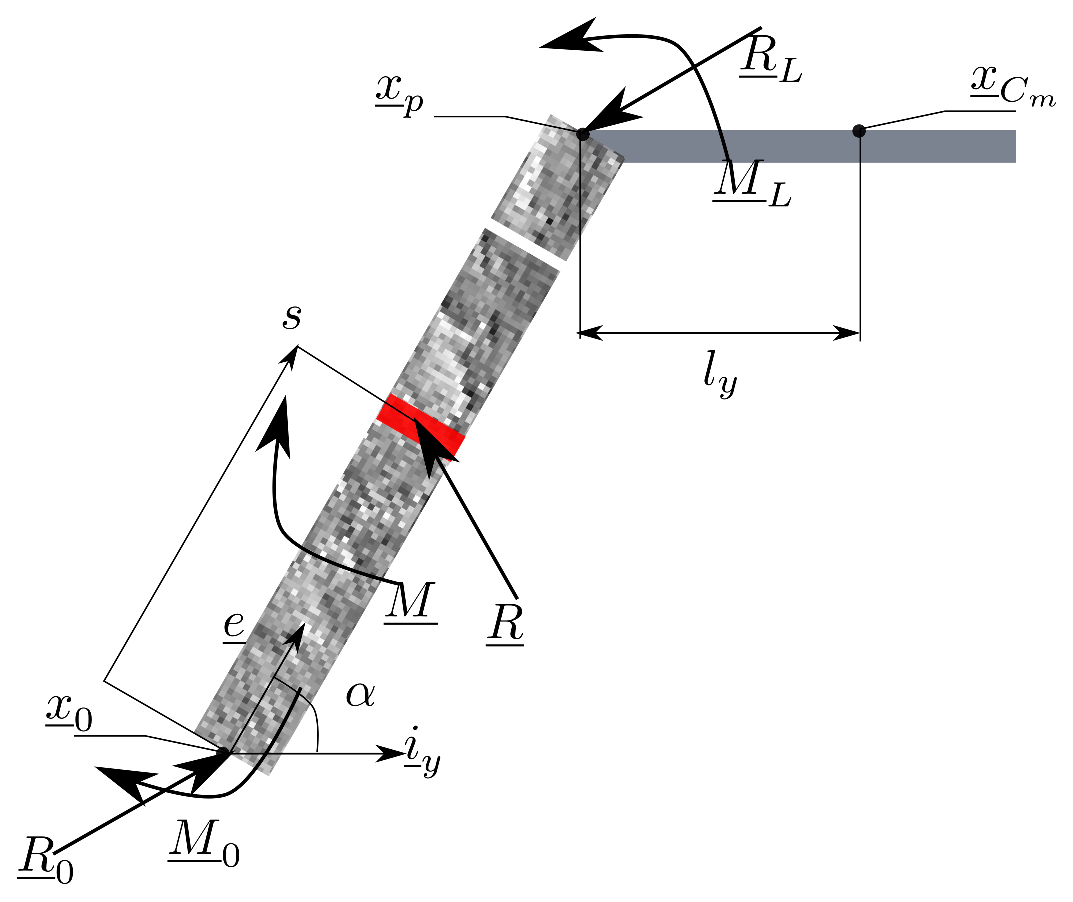
\includegraphics[width=40mm]{moving_crane_1.eps}
\end{center}

	}
\end{frame}


\section{Hands on session}
\subsection{6.2 Moving Crane}
\label{sec:moving_crane}
\framecard{6.2 Moving Crane}
\begin{frame}{Set up}
	\bfc{\igwf{configuration_moving_crane.eps}{75mm}}{Set up [Credits: G. Puel]}{}
\end{frame}


% Set up
\begin{frame}{Set up}
	\txb{120}{3}{12}{
		\begin{block}{Static case }
{			\scriptsize
\begin{itemize}
	\item Support: $\Omega_0 (s=0)$
	\item Crane: $\Omega$\\ axis: $\vct{e}{}{},\pscl{\ebv}{\iz}=\cos\alpha, \pscl{\ebv}{\iy}=\sin\alpha, \alpha\in\psp{0,\frac{\pi}{2}}$\\ geometry: $s\in\left]0,L\right[$, cross-section area $A$,\\ cross-section geometric moment of inertia $\tens{J}{}{}= I \tens{I}{}{}+ \left(J - I\right) \vct{e}{}{}\otimes\vct{e}{}{}$ \\ material properties: $E$, $\mu$\\
	distributed load: $\fv[L]=\zerov$
	\item Rigid horizontal plate $\Omega_p$:\\
	clamping in $\xv[p] (s=L)$, center of mass $\xv[C_m]=\xv[p]+l_x\ix+l_y\iy+l_z\iz$
\end{itemize}              }                                                                              \end{block}
\begin{center}
	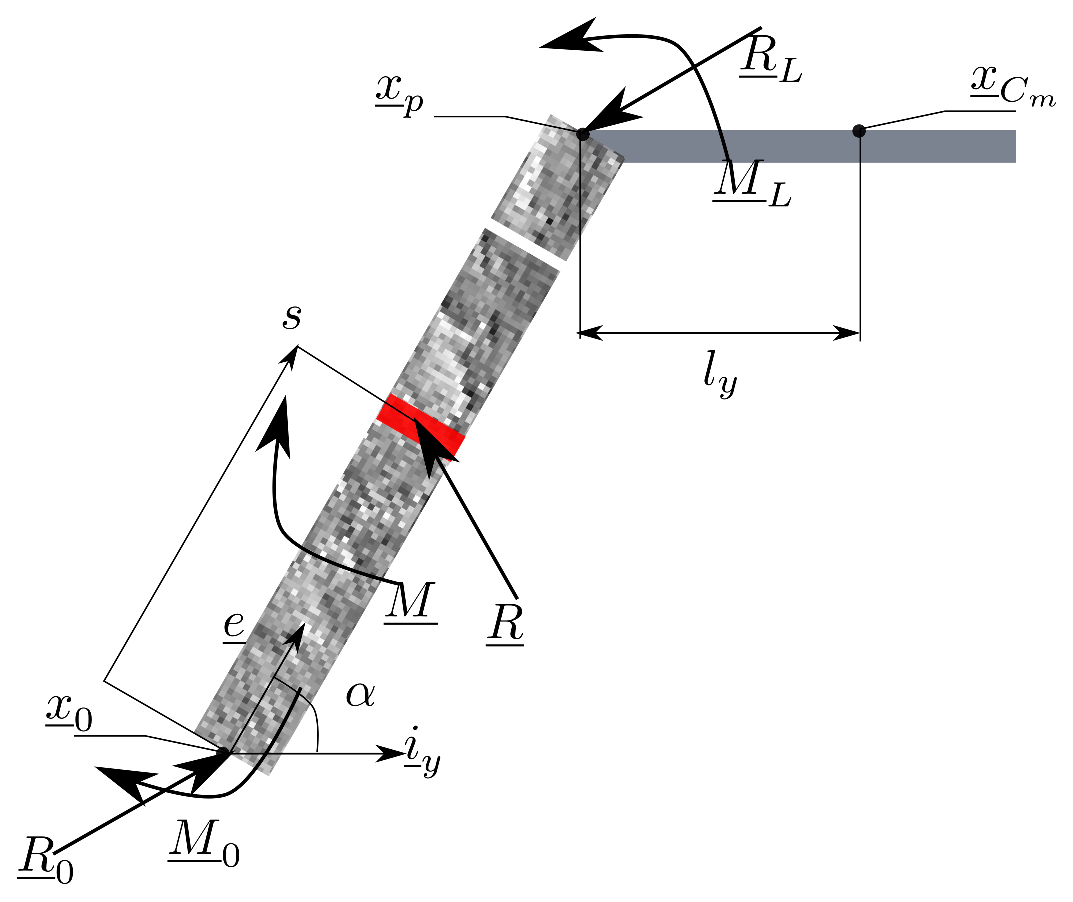
\includegraphics[width=40mm]{moving_crane_1.eps}
\end{center}

	}
\end{frame}


\begin{frame}{Plate balance}
	\txb{120}{3}{12}{
		\begin{exampleblock}{Question 1: Balance of the horizontal plate $\Omega_p$}
			\begin{itemize}
				\item $-\Rv[L]-m g\iz=\zerov \Rightarrow \Rv[L]=\Rv(L)=-mg\iz$
				\item $-\Mv[L]+\pdp{\xv[C_m]-\xv[p]}\wedge(-m g\iz)=\zerov \Rightarrow \Mv[L]=\Mv(L)=mg(l_x\iy-l_y\ix)$
		\end{itemize}                                                                                     \end{exampleblock}
	\begin{center}
	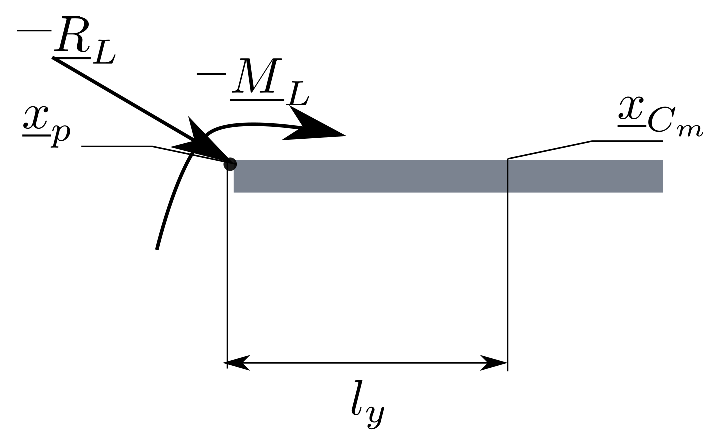
\includegraphics[width=40mm]{moving_crane_2.eps}
	\end{center}

	}

\end{frame}


\begin{frame}{Crane balance}
	\txb{120}{3}{12}{
		\begin{exampleblock}{Questions 2/3: Balance of the moving crane $\Omega$}
			\begin{itemize}
				\item $-\Rv(s)+\Rv[L]=\zerov \Rightarrow \Rv(s)=\Rv[L]=\Rv(L)=-mg\iz$
				\item $-\Mv(s)+\Mv[L]+\pdp{\xv[p]-\xv}\wedge\Rv[L]=\zerov \Rightarrow -\Mv(s)+\Mv[L]+\pdp{L-s}\ebv\wedge(-mg\iz)$\\
				$\Mv(s)=mg(l_x\iy-l_y\ix)+mg\sin\alpha(s-L)\ix$
		\end{itemize}                                                                                     \end{exampleblock}
		\begin{center}
			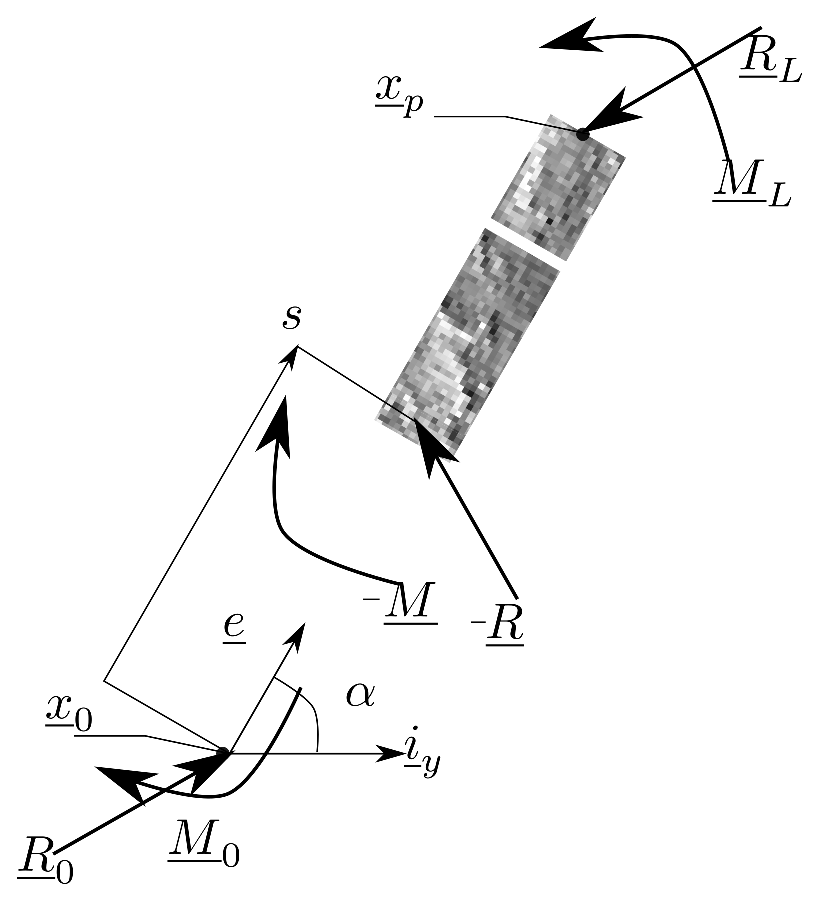
\includegraphics[width=40mm]{moving_crane_3.eps}
		\end{center}
	}
\end{frame}



%\section{Modélisation du comportement mécanique}
%\subsection{Hypothèses fondamentales}
\label{subsec:modelling_hypothesis}
\framecard{Hypothèse fondamentales}
\begin{frame}{Généralités}
\begin{enumerate}
\item Relation entre contraintes et déformations (et/ou leur taux) \\
$ \stress \longleftrightarrow \strain$ ??
\item Nécessité d'un état de contraintes (déformations) homogènes, sans
localisation des déformations
\item Nécessité de définir les domaines de comportement\\
Élasticité vs. Plasticité vs. Viscosité ??
\item Nécessité des expériences au laboratoire
\item Représentatif des conditions in-situ
\item Chemin de chargement
\item Rôle de l'existence de l'eau
\end{enumerate}
\end{frame}

\begin{frame}{Hypothèses fondamentales}
\begin{itemize}
	\item Cinématique linéarisée : formulation en petites déformations \\ $$\strain=\frac{1}{2}\pdp{\gradt{u}{x}{}+\gradt{u}{x}{T}}$$
	$\vct{u}{}{}$ continu en espace/temps
	\item Milieux saturé d'eau (pression d'eau $u_w$) $\to$ contraintes effectives:
	\beq{\stress = u_w\ID+\stress[][,]}{effective-stress}
	$\stress[][,]$ et $u_w$ continus en espace/temps
\item Pas d'influence de la vitesse de sollicitation:
\beq{\stress[][,] = \mathcal{F}\pdp{\strain,\chih},\quad \chih \text{ variables statiques d’écrouissage}}{stress-strain-generic}
\item Conditions isothermes $$T=const.$$
\end{itemize}
\end{frame}

\begin{frame}{Domaines de comportement}
\bfc{\subfh{strain-stress-traction-ex}{30mm}{}\subfh{elastic-domain}{30mm}{}}{\beq{\strain=\strainel+\strainpl}{strainelpl}}{assumptions}
\only<1>{
\begin{itemize}
	\item $\strainel$ sont réversibles (récupérées après décharge)
	\item $\strainpl$ sont irréversibles (non récupérées après décharge)
\end{itemize}
}
\only<2>{
\begin{itemize}
	\item Comportement Élastique (réversible) : $f<0$
	\item Écoulement Plastique (irréversible) : $f=0$
	\item $f$ définie dans l'espace de contrainte mais elle varie avec écoulement plastique (écrouissage)
\end{itemize}
}
\end{frame}

\begin{frame}{Questions ouvertes}
\begin{itemize}
	\item Comment définir le limite élastique en fonctions de contraintes $f\pdp{\stress}$?
	\item Quel repère utiliser?
\item Comment définir différent mécanisme (volumétrique, cisaillement etc)?
\item Comment définir l'écrouissage (évolution non-linéaire de $f$) $$\delta f = df\pdp{\stress,\chih}=\gradfstress:\dstress+\gradfhidd:\dchih$$
\end{itemize}
\end{frame}

\begin{frame}{Exemple d'écrouissage cyclique}
\begin{textblock}{125}(2,10)
	\begin{figure}
		\begin{center}
			\animategraphics[height=65mm,keepaspectratio,autoplay,loop,poster,loop]{1}{deviator_plane_}{0}{3}
		\end{center}
	\end{figure}
	\textbf{Limit strength :} \fbox{$\boldsymbol{\tau_{max} = \frac{C}{\kappa}+\sigma_{yld}}$} 
\end{textblock}
\end{frame}
%\subsection{Stress tensor decomposition}
\label{subsec:stress-decomposition}
\framecard{Stress tensor decomposition}
\begin{frame}{$\stress$ : principal directions}
\only<2>{
\txb{125}{0}{55}{
\centering
\begin{itemize}
	\item Real symmetric stress tensor: $\stress=\stress[][T]\in\mathbb{R}^{(d+1)d/2}$\\$\to\exists$ orthonormal basis of eigenvectors $\phiv[k]$
	\item Principal directions :\vspace{-2mm}
	 \beqh[\stress\pxtp\phiv[k\pxtp]=\lambda_k^\dsigma\pxtp\phiv[k]\pxtp][es][<1-2>][XYZ]
	$\to \tauvsigma=\zerov$ along principal directions!
\end{itemize}
}
}
\txb{55}{0}{13}{
\igwf{decomposition-stress}{55mm}
}
\txb{65}{60}{13}{
	Facet $\Sigma$ oriented along $\nv$\vspace{-2mm}
 \beq{\stress\pxtp.\nv=\stressnn\nv\pxtp+\tauvsigma\pxtp}{stressdec}\vspace{-2mm}
 Normal traction component:\vspace{-2mm} \beq{\pscl{\nv}{\stress.\nv}\pxtp=\stressnn\pxtp}{stressnn}\vspace{-2mm}
 Tangential traction component (shearing)\vspace{-2mm} \beq{\tauvsigma\pxtp=\stress\pxtp-\stressnn\nv\pxtp}{tausigma}
}
\end{frame}

\begin{frame}{$\stress$ Principal directions (2D)}

\txb{55}{0}{13}{
	\igwf{decomposition-stress-2D}{55mm}\\
	\igwf{Mohr-circles1}{35mm}
}
\txb{65}{60}{13}{
	Principal direction = Simple traction\vspace{-2mm}
	\beq{\stress=\dsigma_{ee}\ebv\otimes\ebv,\quad\pscl{\ebv}{\nv}=\cos \alpha}{tracsimple}\vspace{-2mm}
	Normal traction component:\vspace{-2mm} \beq{\stressnn=\frac{\dsigma_{ee}}{2}\pdp{1+\cos 2\alpha}}{stressnn-ts}\vspace{-2mm}
	Tangential traction component (shearing)\vspace{-2mm} \beq{\norm{\tauvsigma}=\vert\pscl{\mv}{\stress.\nv}\vert=\vert\frac{\dsigma_{ee}}{2}\sin 2\alpha\vert}{tausigma1}
	$\pdp{\stressnn,\norm{\tauvsigma}}$: 2D Mohr's circle
}
\only<2>{
\txb{125}{0}{65}{
	In 3D $\to$:
	\beq{
		\begin{split}
\stress\pxtp\phiv[k\pxtp]=\lambda_k^\dsigma\pxtp\phiv[k]\pxtp\\
\det\pdp{\stress-\lambda_k^\dsigma\ID}=0\to -(\lambda_k^\dsigma)^3+I_1\pdp{\stress}(\lambda_k^\dsigma)^2-I_2\pdp{\stress}\lambda_k^\dsigma+I_3\pdp{\stress}=0
		\end{split}		
	}{eigenstress}
}
}
\end{frame}

\begin{frame}{$\stress$ Invariants}

\txb{55}{0}{10}{
	\igwf{principal-stress}{20mm}\igwf{Mohr-circle3}{30mm}
}
\txb{70}{55}{11}{
	\beq{\stressnn=\frac{\lambda^\dsigma_K+\lambda^\dsigma_L}{2}+\frac{\lambda^\dsigma_K-\lambda^\dsigma_L}{2}\cos2\alpha}{}
	\beq{\norm{\tauvsigma}=\frac{\lambda^\dsigma_K-\lambda^\dsigma_L}{2}\vert\sin2\alpha\vert}{}
}
\only<2>{
\txb{125}{2}{36}{
	\beq{I_1\pdp{\stress}=Tr\pdp{\stress}=\ID:\stress=\sum_{i=1}^3\dsigma_{ii}=\sum_{k\in\pbp{I,II,III}}\lambda_k^\dsigma}{I1stress}\vspace{-4mm}
	\beq{I_2\pdp{\stress}=\frac{Tr\pdp{\stress}^2-Tr\pdp{\stress[][2]}}{2}=\lambda_1^{\dsigma}\vspace{-1mm} \lambda^{\dsigma}_2+\lambda_2^{\dsigma}\lambda^{\dsigma}_3+\lambda_1^{\dsigma}\lambda^{\dsigma}_3}{I2stress}\vspace{-1mm}
	\beq{I_3\pdp{\stress}=\frac{1}{3}Tr\pdp{\stress[][3]}=\det\pdp{\stress}}{I3stress}\vspace{-1mm}
	\beq{I_n\pdp{\stress}=\frac{1}{n}Tr\pdp{\stress[][n]}=\det\pdp{\stress}}{Instress}
	Les invariants ne dépendants pas de base choisie
}
}
\end{frame}

\begin{frame}{$\stress$ Mohr's circles}
\only<1>{
\txb{125}{2}{13}{
	\begin{itemize}
		\item $\nv=\sum_{i\in\pbp{I,II,III}} n_i \Phibv[i]$
		\item $\norm{\nv}^2=\sum_{i\in\pbp{I,II,III}} n_i^2=1$
		\item $\stress.\nv=\sum_{i\in\pbp{I,II,III}}\lambda^\dsigma_k n_k\Phibv[k]$
		\item $\stressnn=\sum_{i\in\pbp{I,II,III}}\lambda^\dsigma_k n_k^2$
		\item $\norm{\stress.\nv}^2=\stressnn^2+\norm{\tauvsigma}^2=\sum_{i\in\pbp{I,II,III}}(\lambda^\dsigma_k)^2 n_k^2$
	\end{itemize}
	\bsys[][
	& n_I^2 =\frac{\norm{\tauvsigma}^2+\pdp{\stressnn-\lambda_{II}^\dsigma}\pdp{\stressnn-\lambda_{III}^\dsigma}}{\pdp{\lambda_I^\dsigma-\lambda_{II}^\dsigma}\pdp{\lambda_I^\dsigma-\lambda_{III}^\dsigma}} \\
	&n_{II}^2 =\frac{\norm{\tauvsigma}^2+\pdp{\stressnn-\lambda_{I}^\dsigma}\pdp{\stressnn-\lambda_{III}^\dsigma}}{\pdp{\lambda_{II}^\dsigma-\lambda_{I}^\dsigma}\pdp{\lambda_{II}^\dsigma-\lambda_{III}^\dsigma}} \\
	&n_{III}^2 =\frac{\norm{\tauvsigma}^2+\pdp{\stressnn-\lambda_{I}^\dsigma}\pdp{\stressnn-\lambda_{II}^\dsigma}}{\pdp{\lambda_{III}^\dsigma-\lambda_{II}^\dsigma}\pdp{\lambda_{III}^\dsigma-\lambda_{II}^\dsigma}} 
	][normal-components]
}
}
\only<2>{\bfc{\ighf{mohr-ex1}{62.5mm}}{Credits J-A. Goulet}{mohr-ex1}}
\only<3>{\bfc{\ighf{mohr-ex2}{62.5mm}}{Credits J-A. Goulet}{mohr-ex2}}
\only<4>{\bfc{\ighf{mohr-ex3}{62.5mm}}{Credits J-A. Goulet}{mohr-ex3}}
\only<5>{\bfc{\ighf{mohr-ex4}{62.5mm}}{Credits J-A. Goulet}{mohr-ex4}}
\only<6>{\bfc{\ighf{mohr-ex5}{62.5mm}}{Credits J-A. Goulet}{mohr-ex5}}
\end{frame}

\begin{frame}{$\stress$ decomposition}
	\vspace{-5mm}
	Every isotropic function $f\pdp{\stress}$ can be expressed as a symmetric function of principal stress components or its invariants. $\stress$ can be decomposed into two parts: $\stress=\dsigma_m\ID+\deviator$
	\begin{enumerate}
		\item Spherical or mean stress:
		\beq{\dsigma_m=\frac{1}{3}\stress:\ID=\frac{1}{3}Tr(\stress)}{avgstress}
		\item Deviatoric stress :
		\beq{\deviator=\stress-\dsigma_m\ID}{devstress}
	\end{enumerate}
Invariants of $\deviator$:
{\scriptsize
\begin{itemize}
	\item \vspace{-2mm}$J_1\pdp{\deviator}=Tr\pdp{\deviator} = 0$\vspace{-2mm}
	\item $J_2\pdp{\deviator}=\frac{1}{2}Tr\pdp{\deviator[][2]}=I_2\pdp{\stress}-\frac{I_1\pdp{\stress}^2}{6} $
	\item\vspace{-2mm} $J_3\pdp{\deviator}=\frac{1}{3}Tr\pdp{\deviator[][3]}=I_3\pdp{\stress}-2\frac{I_1\pdp{\stress}J_2\pdp{\deviator}}{3}+\frac{I_1^3\pdp{\stress}}{27}$
\end{itemize}
}
\end{frame}


\begin{frame}{$\stress$ decomposition}
 	Every isotropic function $f\pdp{\stress}$ can be expressed as a symmetric function of \stress principal components, or its invariants $I_1,J_2,J_3$, and of $\deviator$.
    \bfc{\ighf{deviatoric-representation}{40mm} \ighf{deviatoric-representation-plane}{40mm}}{Adapted from Potts et Zdravkovic, 1999}{deviatoric-representation}
\end{frame}

\begin{frame}{Haigh-Westergaard coordinates}
\only<1>{
\begin{itemize}
	\item Haigh-Westergaard decomposition:
	\beq{\stress=\pdp{\Pt[z]:\stress}\Pt[z]+\pdp{\Pt[r]:\stress}\Pt[r]}{}
	\item Projection on hydrostatic axis:
	\beq{\begin{split}
&\xi=\Pt[z]:\stress=\sqrt{3}\dsigma_m\\ &\Pt[z]=\frac{\ID}{\norm{\ID}}=\frac{\ID}{\sqrt{3}}=\sum_{k\in\pbp{I,II,III}}\nv[k]\otimes\frac{\nv[k]}{\sqrt{3}}
		\end{split}}{xi-hw}
\end{itemize}
}
\only<2>{
\begin{itemize}
	\item Projection onto deviatoric axis:
	\beq{\Pt[r]:\stress=\norm{\deviator}=\sqrt{2J_2\pdp{\deviator}}=\rho\to\rho\Pt[r]=\deviator}{rho-hw}
	\item Principal direction of the deviatoric stress:
	{\scriptsize
	\beq{\Pt[r]=\frac{1}{\rho}\sqrt{\frac{2}{3}}\sum_{k\in\pbp{I,II,III}}\pdp{\stress.\gv[k]}\otimes\gv[k]=\frac{1}{\rho}\deviator\quad \gv[k]\otimes\gv[k]=\sqrt{\frac{3}{2}}\pdp{\nv[k]\otimes\nv[k]-\frac{1}{3}\ID}
%		\begin{split}
%			\deviator\frac{\nv[k]}{\sqrt{3}}=\pdp{\lambda^{\dsigma}_k-\dsigma_m}\frac{\nv[k]}{\sqrt{3}} = \pdp{\lambda^{\dsigma}_k-\xi}\nv[k]\\
%			\vct{g}{k}{}=\sqrt{\frac{3}{2}} \pdp{\nv[k]-\Pt[z]\nv[k]}=
%		\end{split}
	}{Pr} 
}
	\item Lode's angle:
	{\scriptsize
\beq{\pscl{\deviator\gv[I]}{\gv[I]}=\sqrt{\frac{2}{3}}\rho\cos\theta\to\theta = \frac{1}{3}arcsin\pdp{\frac{J_3\pdp{\deviator}}{2}\pdp{\frac{2}{J_2\pdp{\deviator}}}^{3/2}}}{LodeAngle}
}
\end{itemize}
}
\end{frame}
%\subsection{Types de chargement}
\label{subsec:types-chargement}
\framecard{Types de chargement}
%\begin{frame}{Compression et cisaillement}
%\bfc{\ighf{chargement}{65mm}}{Chemins classiques de chargement}{chargement}
%\end{frame}

\begin{frame}{Chemins de chargement}
\begin{itemize}
\item Compression:
\begin{enumerate}
\item Compression isotrope \hyperlink{frame:comp-iso}{\beamerbutton{GOTO}}
\item Compression odeométrique \hyperlink{frame:comp-oedo}{\beamerbutton{GOTO}}
\end{enumerate}
\item Cisaillement
\begin{enumerate}
	\item triaxial de révolution \hyperlink{frame:triax-revo}{\beamerbutton{GOTO}}
	\item torsion cylindre plein \hyperlink{frame:tors-pleine}{\beamerbutton{GOTO}}
	\item torsion cylindre creux  \hyperlink{frame:tors-hollow}{\beamerbutton{GOTO}} 
	\item cisaillement simple
	\item vrai triaxial
\end{enumerate}
\end{itemize}
Questions supplémentaires:
\begin{itemize}
	\item Avec rotation des directions principales
\item Sans rotation des directions principales
\item Influence de la pression interstitielle (drainé, non-drainé)
\item composantes contrôlées (imposées)/composantes mesurées
\end{itemize}
\end{frame}

\begin{frame}{\hypertarget{frame:comp-iso}{Compression isotrope}}
\bfc{\ighf{compression-iso}{35mm}\ighf{example-iso}{40mm}{}}{\cite{Book_Bardet_1997_Experimental_soil_mechanics}}{example-oedo}
$\depsil_V=3\depsil_1=Tr\pdp{\strain}$ déformation volumique
\end{frame}

\begin{frame}{\hypertarget{frame:comp-oedo}{Compression odeométrique}}
\ighf{chemin-oedometrique}{35mm}\\
\bfc{\ighf{example-oedo}{30mm}{}}{\cite{Book_Bardet_1997_Experimental_soil_mechanics}}{example-oedo}
\end{frame}

\begin{frame}{\hypertarget{frame:triax-revo}{Triaxial de révolution}}
\only<1>{\ighf{example-triax-rev}{65mm}
$$\rho=\sqrt{2J_2\pdp{\deviator}}=\sqrt{\frac{2}{3}}q$$}
\only<2>{\ighf{options-triax-rev}{65mm}}
\end{frame}

\begin{frame}{\hypertarget{frame:tors-pleine}{Torsion cylindre plein}}
\only<1>{
	\bfc{\ighf{example-tors-pleine}{65mm}}{\cite{Shimizu_et_al_2009}}{example-tors-pleine}
}
\only<2>{
\txb{60}{2}{13}{
	\bfc{\ighf{example-tors-pleine}{32mm}}{\cite{Shimizu_et_al_2009}}{example-tors-pleine}
}
\txb{63}{60}{13}{
	$\forall \pdp{\theta,z}\in]0,2\pi[\times]0,H[$:
	$$\stress\pxtp=2kr\ibv[\theta]\pdp{\theta}\otimes_s\ibv[z]$$
	$$Div_x\stress\pxtp=0$$
	$$\stress\pdp{r=\frac{D}{2},\theta,z}.\ibv[r]\pdp{\theta}=0$$
}
\txb{125}{0}{55}{
	$$\vct{F}{}{}\Big\vert_{z=H}=\int_{0}^{2\pi}\int_{0}^{\frac{D}{2}}\stress\pdp{r,\theta,z=H}.\ibv[z] r dr d\theta=0$$
	$$\vct{M}{0}{}\Big\vert_{z=H}=\int_{0}^{2\pi}\int_{0}^{\frac{D}{2}}r\ibv[r]\wedge\stress\pdp{r,\theta,z=H}.\ibv[z] r dr d\theta=M_t \ibv[z]\to k=\frac{32 M_t}{\pi D^4}$$
	$$\lambda_{I,II,III}^\dsigma=\pbp{-kr,0,kr}\to \tau_{max}=\frac{kD}{2}=\frac{16 M_t}{\pi D^3}$$
}
}
\end{frame}


\begin{frame}{\hypertarget{frame:tors-hollow}{Torsion cylindre creux}}
\only<1>{
\bfc{\ighf{example-tors-hollow}{65mm}}{\cite{Fukuda_2014}}{example-tors-hollow}
}
\only<2-3>{
\txb{60}{2}{13}{
	\bfc{\ighf{example-tors-hollow}{32mm}}{\cite{Fukuda_2014}}{example-tors-hollow}
}
\txb{63}{60}{13}{
	$\forall \pdp{\theta,z}\in]0,2\pi[\times]0,H[, $\\
	$p_e<0,p_i<0, \frac{D}{e}\ggg1$:
	$$\stress\pxtp=2kr\ibv[\theta]\pdp{\theta}\otimes_s\ibv[z]+$$ $$+\frac{\pdp{p_i+p_e}\pdp{\frac{D}{2}-r}-p_e e}{e}\ibv[r]\pdp{\theta}\otimes\ibv[r]\pdp{\theta}$$
	$$Div_x\stress\pxtp=0$$
}
\txb{125}{0}{55}{
\only<2>{
$$\stress\pdp{r=\frac{D}{2},\theta,z}.\ibv[r]\pdp{\theta}=p_e\ibv[r]$$
$$\stress\pdp{r=\frac{D}{2}-e,\theta,z}.-\ibv[r]\pdp{\theta}=-p_i\ibv[r]$$
}
\only<3>{
	$$\vct{F}{}{}\Big\vert_{z=H}=\int_{0}^{2\pi}\int_{\frac{D}{2}-e}^{\frac{D}{2}}\stress\pdp{r,\theta,z=H}.\ibv[z] r dr d\theta=0$$
	$$\vct{M}{0}{}\Big\vert_{z=H}=\int_{0}^{2\pi}\int_{\frac{D}{2}-e}^{\frac{D}{2}}r\ibv[r]\wedge\stress\pdp{r,\theta,z=H}.\ibv[z] r dr d\theta=M_t \ibv[z]\to k\underset{D/e\ggg 1}{\approx}\frac{2 M_t}{\pi e D^3}$$
	$$\lambda_{I,II,III}^\dsigma=\pbp{-kr,0,kr}\to \tau_{max}=\frac{kD}{2}=\frac{ M_t}{\pi e D^2}>\frac{16 M_t}{\pi D^3} \iff \frac{D}{e}\ggg 16$$
}
}
}
\end{frame}
%
%\section{Élasticité et rupture}
%\subsection{Linear Elasticity}
\label{subsec:elasticity}
\framecard{Linear Elasticity}
%\begin{frame}{Comportement typique des sols}
%\txb{123}{2}{9}{
%\centering
%\bfc{\subfw{triaxial-sample}{15mm}{}\subfh{elastic-modula-ep}{35mm}{}\subfh{ep-example}{35mm}{}
%}{Chargement triaxiale et évolution du déviateur $q$ en fonction de la déformation axiale $\depsil_1$. Comportement élasto-plastique (b) et élasto-plastique parfait.}{elastic-modula}
%}
%\txb{125}{0}{70}{
%\begin{itemize}
%	\item $E_i$ : module de Young \textit{initial} 
%	\item $E_t$ : module de Young \textit{tangent} 
%	\item $E_s$ : module de Young \textit{sécant} 
%\end{itemize}
%}
%\end{frame}


\begin{frame}{Elasticity theory}
\txb{123}{2}{11}{
	$\stress\pxtp=\mathcal{F}\pdp{\strainel\pxtp}$
	\begin{itemize}
		\item<only@2> Linearity $\to g\pdp{\alpha\strainel[1]+\beta\strainel[2]}=\alpha\mathcal{F}\pdp{\strainel[1]}+\beta\mathcal{F}\pdp{\strainel[2]}$: 
		\begin{itemize}
			\item Stiffness: \beq{\stress\pxtp=\Del\pdp{\xv} : \strainel\pxtp}{el-stiff-del}
			\item Compliance: \beq{ \strainel=\Cel\pdp{\xv}:\stress\pxtp}{el-comp-cel}
		\end{itemize}
	$\tensf{A}{}{}$: 4$^{th}$-order tensor (real symmetric)\\
	$\tensf{A}{}{}=\tens{A}{l}{}\otimes\tens{A}{r}{},\quad \tensf{A}{}{}:\tens{B}{}{}=\tens{A}{l}{}Tr\pdp{\tens{A}{r}{T}\tens{B}{}{}}$
		\item<only@3> Isotropic $\pbp{\IDD,\ID\otimes\ID}$:
		\begin{itemize}
			\item Stiffness : \beq{\stress\pxtp=\lambda\pdp{\xv}Tr\pdp{\strainel\pxtp}\ID+2\mu\pdp{\xv} \strainel\pxtp }{el-stiff}
			\beq{\Del\pxp=\lambda\pxp\ID\otimes\ID+2\mu\pxp \IDD }{Del_tens}
			\item Compliance: \beq{\strainel\pxtp=\frac{1+\nu\pdp{\xv}}{E\pdp{\xv}}Tr\pdp{\stress\pxtp}\ID-\frac{\nu\pdp{\xv}}{E\pdp{\xv}} \stress\pxtp }{el-comp}
			\beq{\Cel\pxp=\frac{1+\nu\pdp{\xv}}{E\pdp{\xv}}\ID\otimes\ID-\frac{\nu\pdp{\xv}}{E\pdp{\xv}}\IDD}{Cel_tens}
		\end{itemize}
	$\IDD=\sum_{i=1}^3\ebv[i]\otimes\ebv[i]\otimes\ebv[i]\otimes\ebv[i]$
	
		\item<only@4>Spherical and deviatoric decomposition:
		\begin{itemize}
				\item Spherical component (pression) $\stressm$: \beq{\stressm\pxtp=\frac{Tr\pdp{\stress}}{3}=\frac{\pdp{3\lambda\pxp+2\mu\pxp}}{3}Tr\pdp{\strainel\pxtp}=K\pxp\evolel\pxtp}{el-stiff-sigmam}
				\item Deviatoric component $\deviator$:
				\beq{\deviator\pxtp=\stress-\stressm\ID=2\mu\pdp{\xv} \strainel-\frac{2}{3}\mu\pxp\evolel\pxtp=2\mu\pxp\eel\pxtp }{el-stiff-dev}
		\end{itemize}
Direct relationship spherical/deviatoric\\
		$\evolel$: volumetric strain\\
			$\eel$: deviatoric strains	\\
			$\ebar=\sqrt{\frac{4}{3}J_2\pdp{\strain}}$: equivalent deviatoric strain
		\item<only@5> Homogeneity:
		\beq{\Del\pdp{\xv}=\Del,\quad\Cel\pdp{\xv}=\Cel}{homo-el}
		\item<only@5>  $\pdp{\lambda,\mu}$: Lam\'e parameters (stiffness)
		\item<only@5>  $\pdp{E,\nu}$ : Young's modulus and Poisson's coefficient (compliance)
		\item<only@5>  $E>0, \mu>0,\quad 3\lambda+2\mu>0,\quad -1<\nu<0.5$
		\item[]<only@5> \beq{\lambda=\frac{\nu E}{\pdp{1+\nu}\pdp{1-2\nu}},\quad \mu=\frac{E}{2\pdp{1+\nu}}}{}
	\end{itemize}
}
\only<6>{
\bfc{\ighf{hom-elastic-matrices}{65mm}}{Elastic tensors with $\pdp{E,\nu}$.}{hom-elastic-matrices}
}
\end{frame}
%
%\begin{frame}{Thermodynamics approach}
%	\txb{123}{2}{11}{
%	Helmholtz free energy \beq{\Psi = \UInt-T Q}{Helmholtz-fe}$\to \dot{\Psi}=\dot{\UInt}-S dT$ and for isothermal conditions  $\to \dot{\Psi}=\dot{\UInt}$\\
%\only<2>{
%	Exploiting PPT and VPP :
%	\beq{\dot{\UInt}=\PExt-\PKin+\dot{Q}=-\PInt+\dot{Q}}{uint-isoth}
%	Adiabatic conditions $\dot{Q}=0$:
%	\beq{\dot{\UInt}=\dot{\Psi}=-\PInt\pdp{\vV}=\int_{\Omega_t}\stress\pxtp:\straindot\pxtp dv_t}{uint-isoth}
%	In isothermal conditions, free-energy corresponds to strain energy: \\
%	$\dot{\UInt }= \int_{\Omega_t}\rho \dot{u} dv_t \to \rho \dot{u}\pxtp = \rho \dot{\psi}\pxtp$
%}
%}
%\end{frame}
%
%\begin{frame}{Stiffness matrix}
%
%	\txb{30}{0}{11}{
%		\igwf{free-energy}{30mm}
%	}
%	\txb{95}{30}{11}{
%		$\rho \psi\pxtp$ integral of curve $\stress\pxtp=\mathcal{F}\pdp{\strain\pxtp}$
%		\\ 
%		$\to\rho\psi\pxtp = \rho \psi_0+\int_{t_0}^{t_0+T}\stress\pxtp:\straindot\pxtp dt = \int_{\strain\pdp{t_0}}^{\strain\pdp{t_0+T}}\stress\pxtp:\dstrain\pxtp$
%		
%	}
%\only<2>{
%\txb{125}{0}{47}{	
%	
%	\beq{\stress\pxtp = \sum_{i,j=1}^3\frac{\partial\pdp{\rho\psi}}{\partial\depsil_{ij}} \ebv[i]\otimes\ebv[j]=\hessian[\depsil]\pdp{\rho\psi} \text{Hessian}}{stress-grad-psi}
%	
%	\beq{\Del\pxtp = \sum_{k,l=1}^3\frac{\partial\stress}{\partial\depsil_{kl}} \otimes \ebv[k]\otimes\ebv[l]=\sum_{i,j,k,l=1}^3\frac{\partial\pdp{\rho\psi}}{\partial\depsil_{ij}\depsil_{kl}}\ebv[i]\otimes\ebv[j]\otimes \ebv[k]\otimes\ebv[l]}{stress-grad-psi}
%	
%}
%}
%\end{frame}
%
%\begin{frame}{Stiffness matrix}
%
%	\txb{123}{2}{11}{	
%		Free-Energy becomes:
%			\beq{\rho\psi=\frac{E}{\pdp{1-2\nu}\pdp{1+\nu}}\pdp{ \pdp{1-2\nu}Tr\pdp{\strain[][2]} +\nu Tr{\strain}^2}}{en-deformation}
%	\beq{
%	\begin{split}
%		& \rho\psi = \frac{\stressm\evol+2\mu \edv:\edv}{2},\quad \rho\delta\psi =\stressm\delta\evol+\deviator:\dedv\\
%		& \rho\psi=\frac{1}{2}K\evol[2]+\frac{3\mu}{2}\ebar[][2],\quad \rho\delta\psi=K\evol\delta\evol+3\mu \ebar\delta\ebar
%	\end{split}
%}{psi-p-dev}
%
%	\beq{
%	\begin{split}
%		& K =\frac{\delta\stressm}{\devol}= \rho \frac{\partial^2\psi}{\partial\evol[2]}\\
%		& 3\mu =\frac{\delta q}{\delta\ebar}= \rho \frac{\partial^2\psi}{\partial\ebar[][2]}
%	\end{split}
%}{K-G-psi}
%
%}
%\end{frame}
%
%\begin{frame}{Summary}
%\centering
%\bfc{\igwf{wood-elasticity-modules}{110mm}}{Adapted from \cite{Book_diPrisco_Wood_Mechanical_Behaviour_Soil_Cyclic}}{wood-elasticity-modules}
%\end{frame}
%
%\begin{frame}{Anisotropic Linear Elasticity}
%	\igwf{elast-aniso}{110mm}
%\end{frame}
%
%\begin{frame}{Non-Linear Elasticity}
%\only<3>{
%	\igwf{ramberg-osgood}{110mm}
%}
%\only<1>{
%\txb{40}{0}{11}{
%	\igwf{el-nlin}{35mm}\\
%}
%\txb{85}{40}{11}{
%$\stress=\Del\pdp{\stress}:\strain\to$ elastic moduli depend on strain but no residual strain (fully reversible).
%\begin{itemize}
%	\item $K=K_{ref}\pdp{\frac{\stressm}{\dsigma{m,ef}}},\mu=\mu_{ref}\pdp{\frac{\stressm}{\dsigma_{m,ref}}},\nu=\text{const.}$
%	\item not coming from a potential
%	\item problems when number of curves is too high
%\end{itemize}
%Hyperbolic model \cite{Duncan_Chang_1970}:
%\beq{
%\begin{split}
%& q = \frac{\depsil_1}{\frac{1}{E_i}+\frac{\depsil_1}{q_{ult}}}\\
%& q_f = R_fq_{ult}=\frac{2c\cos\phi+2\dsigma_3\sin\phi}{1-\sin\phi}
%\end{split}
%}{duncan-cheng}
%$q=\dsigma_1-\dsigma_3$\\
%$R_f$: ratio admissible deviatoric stress/Coulomb strength
%}
%}
%
%
%\only<2>{
%	\txb{40}{0}{11}{
%		\igwf{el-nlin}{35mm}\\
%	}
%	\txb{85}{40}{11}{
%		Incremental linear elasticity:
%		\begin{itemize}
%				\item $E_i=k\pdp{\frac{\dsigma_3}{p_a}}^n$
%			\item $K_i=k_b\pdp{\frac{\dsigma_3}{p_a}}^m$
%			\item $E_t=E_i\pdp{1-R_f\frac{\pdp{1-\sin\phi}q}{2c\cos\phi+2\dsigma_3\sin\phi}}^2$
%		\end{itemize}
%}}
%\end{frame}


%THE END


%\begin{frame}{Approche thermodynamique}
%\txb{123}{2}{11}{
%	Énergie libre de Gibbs \beq{\GGibbs = \Hent  -T Q}{Gibbs-fe}\\
%	Enthalpie $\Hent=\UInt-\int_{\Omega_t}$
%	$\to \dot{\Psi}=\dot{\UInt}-S dT$ et dans le cas isotherme  $\to \dot{\Psi}=\dot{\UInt}$\\
%	\only<2>{
%		En utilisant le PPT (\Cref{eq:tdp1}) et le PPV (\Cref{eq:VPP}), on obtient:
%		\beq{\dot{\UInt}=\PExt-\PKin+\dot{Q}=-\PInt+\dot{Q}}{uint-isoth}
%		Dans le cas isotherme (adiabatique) $\dot{Q}=0$:
%		\beq{\dot{\UInt}=\dot{\Psi}=-\PInt\pdp{\vv}=\int_{\Omega_t}\stress\pxtp:\straindot\pxtp dv_t}{uint-isoth}
%		En conditions isothermes, l’énergie libre est uniquement une énérgie de déformation: \\
%		$\UInt = \int_{\Omega_t}\rho u dv_t \to \rho u\pxtp = \rho \psi\pxtp$
%	}
%}
%\end{frame}
%
%
%\begin{frame}{Matrices de souplesse (cond. isothermes)}
%
%\txb{30}{0}{11}{
%	\igwf{compl-energy}{30mm}
%}
%\txb{95}{30}{11}{
%	$\rho e_c\pxtp$ intégral de la courbe $\strain\pxtp=\mathcal{F}\pdp{\strain\pxtp}$
%	\\ 
%	$\to\rho\psi\pxtp = \rho \psi_0+\int_{t_0}^{t_0+T}\stress\pxtp:\straindot\pxtp dt = \int_{t_0}^{t_0+T}\stress\pxtp:\dstrain\pxtp$
%	
%}
%\only<2>{
%	\txb{125}{0}{47}{	
%		
%		\beq{\stress\pxtp = \sum_{i=1}^3\sum_{j=1}^3\frac{\partial\pdp{\rho\psi}}{\partial\depsil_{ij}} \ebv[i]\otimes\ebv[j]=\hessian[\depsil]\pdp{\rho\psi} \text{Hessian}}{stress-grad-psi}
%		
%		\beq{\Del\pxtp = \sum_{k=1}^3\sum_{l=1}^3\frac{\partial\stress}{\partial\depsil_{kl}} \otimes \ebv[k]\otimes\ebv[l]=\sum_{k=1}^3\sum_{l=1}^3\frac{\partial\pdp{\rho\psi}}{\partial\depsil_{ij}\depsil_{kl}}\ebv[i]\otimes\ebv[j]\otimes \ebv[k]\otimes\ebv[l]}{stress-grad-psi}
%	}
%}
%%\txb{30}{0}{47}{
%%	\igwf{free-energy}{30mm}
%%}
%%\txb{95}{30}{53}{
%%	$\UInt = \int_{\Omega_t}\rho u dv_t \to \rho u\pxtp = \rho \psi\pxtp$ intégral de la courbe $\stress\pxtp=\mathcal{F}\pdp{\strain\pxtp}$
%%	\\ 
%%	$\to\rho\psi\pxtp = \rho \psi_0+\int_{t_0}^{t_0+T}\stress\pxtp:\straindot\pxtp dt = \int_{t_0}^{t_0+T}\stress\pxtp:\dstrain\pxtp$
%%}
%\end{frame}
%\subsection{Failure Criteria}
\label{subsec:failure-criteria}
\framecard{Failure Citeria}
\begin{frame}{Rupture}
\txb{120}{5}{10}{\vspace{-7mm}\centering
	\bfc{\subfh{eprouvette-traction-ex}{30mm}{}\subfh{boundary-influence-traction-ex}{30mm}{}\\\subfh{strain-stress-traction-ex1}{30mm}{ductile}\subfh{strain-stress-rupture-ex}{30mm}{fragile}\subfh{fragile-ductile-ex}{30mm}{}}{Credits G. Puel}{failure-intro}
}
\end{frame}

\begin{frame}{...at atomistic level}
\txb{120}{5}{10}{\vspace{-7mm}\centering
	\bfc{\subfh{dislocation-ex}{30mm}{}\\\subfh{dislocation-ex1}{30mm}{}}{Credits G. Puel}{dislocation}
}
\end{frame}

\begin{frame}{Splitting failure}
\begin{itemize}
\item Separation of two atomic planes
\item Driven by normal stress component $\stressnn$ 
\item Random atomic planes \\ $\to$ orientation that maximizes $\stressnn$
\beq{f\pdp{\stress}=\max_{\norm{\nv}=1}\stressnn\pxtp-\dsigma_r\leq0}{clivage}
\item for fragile materials (concrete)
\end{itemize}
\bfc{\subfh{clivage}{17.5mm}{}\subfh{brazilian-test}{17.5mm}{}}{Credits G. Puel}{clivage}
\end{frame}

\begin{frame}{Shear failure}
\begin{itemize}
	\item plastic shearing along a certain plane
	\item induced by shearing stress overruns the threshold (Schmidt's law)
	$\stressnn$
\end{itemize}
\only<1>{
\begin{enumerate}
	\item maximum tangent traction component $\to$ Tresca's criterion
	\beq{
		\begin{split}
			& f\pdp{\stress}=\max_{\norm{\nv}=1}\norm{\tauvsigma}\pxtp-\tau_0\leq0\\
			& \nv=\frac{1}{\sqrt{2}}\pdp{\nv[I]+\nv[III]}
		\end{split}	
}{tresca}
\end{enumerate}
\bfc{\subfh{tresca}{17.5mm}{}}{Credits G. Puel}{tresca}
}
\only<2>{
	\begin{enumerate}
		\item Potential energy of elastic distortion $\to$ Von Mises criterion
		\beq{
			\begin{split}
				& f\pdp{\stress}=\dsigma_{eq}-\tau_0\leq0,\quad \dsigma_{eq}=\sqrt{3J_2\pdp{\deviator}}\\
				& \stress=\dsigma_{ee}\ebv[]\otimes\ebv[]\to\dsigma_{eq}=\dsigma_{ee}\\
				& \stress=\tau_{em}\ebv[]\otimes_s\mv[]\to\dsigma_{eq}=\sqrt{3}\tau_{em}
			\end{split}	
		}{mises}
	\end{enumerate}
\bfc{\ighf{tresca-mises-mohr}{17.5mm}{}}{Credits G. Puel}{tresca-mises-mohr}
}
\end{frame}

%\begin{frame}{Soil failure criteria}
%\only<1>{
%\txb{58}{2}{33}{
%	\bfc{\igwf{coulomb}{58mm}}{\cite{Han_et_al_2006}}{coulomb}
%}
%\txb{100}{0}{13}{
%\beq{f\pdp{\stress}=\frac{\vert\lambda_I^\dsigma-\lambda_{III}^\dsigma\vert}{2}-\frac{\lambda_I^\dsigma+\lambda_{III}^\dsigma}{2}\sin\phi-c\cos\phi<0}{coulomb}
%}
%\txb{65}{60}{30}{
%\begin{itemize}
%	\item For granular materials:  positive compression
%	\item Friction failure: Coulomb's law
%	\item $\phi$ friction angle
%	\item $c$ apparent cohesion 
%\end{itemize}
%}
%}
%\only<2>{
%\txb{58}{2}{33}{
%	\bfc{\igwf{coulomb}{58mm}}{\cite{Han_et_al_2006}}{coulomb}
%}
%\txb{100}{0}{13}{
%	\beq{f\pdp{\stress}=\sqrt{J_2\pdp{\stress}}-M\cdot I_1\pdp{\stress}-N\leq0,\quad M=\frac{6\sin\phi}{3-\sin\phi}}{dprager}
%}
%\txb{65}{60}{30}{
%	\begin{itemize}
%		\item Drucker-Prager's criterion
%	\end{itemize}
%}
%}
%\only<3>{
%	\txb{58}{2}{33}{
%		\bfc{\igwf{criteres-duncan-lade}{58mm}}{\cite{Han_et_al_2006}}{criteres-duncan-lade}
%	}
%	\txb{100}{0}{13}{
%		\beq{f\pdp{\stress}=I_1^3\pdp{\stress}-kI_3\pdp{\stress}}{lade-duncan}
%	}
%	\txb{65}{60}{30}{
%		\begin{itemize}
%			\item For sands
%			\item Duncan's criterion
%		\end{itemize}
%	}
%}
%\end{frame}
%
%\begin{frame}{Résumé}
%\txb{125}{0}{13}{
%\bfc{\subfh{compare-failure-criteria-3d}{50mm}{}\subfh{compare-failure-criteria-2d}{25mm}{}}{\cite{Book_Nova_2010_Soil_Mechanics}}{compare-failure-criteria}
%}
%\end{frame}
%
%\begin{frame}{Résumé}
%\txb{123}{2}{13}{
%	\centering
%\bfc{\centering\ighf{compare-failure-criteria-table}{60mm}}{Comparaison entre différent critères de rupture par cisaillement}{compare-failure-criteria-table}
%}
%\end{frame}
%\section{Élastoplasticité}
%\subsection{Élastoplasticité}
\label{subsec:elasto-plasticity}
\framecard{Élastoplasticité}
\begin{frame}{Comportement post-élastique}
	\begin{itemize}
		\item le sol entre en rupture si soumit à une déformation déviatorique relevant ou à traction 
		\item normalement la réponse du sol est non linéaire et irréversible 
		\item le sol peut avoir des déformations volumiques importants quand les
		déformations déviatoriques augmentent
		\item le comportement du sol est dépendant de son histoire
	\end{itemize}

\end{frame}

\begin{frame}{Problème élastoplastique}
\txb{125}{0}{11}{
	\begin{itemize}
		\item Ingrédients pour décrire l'évolution élastoplastique?
	\begin{enumerate}
		\item<only@2> Seuil de plasticité
		\item<only@3>  Fonction de charge (critère de rupture)
		\item<only@4-5> écrouissage (évolution du seuil de plasticité)
		\item<only@6> écoulement plastique
		\item<only@7> problème d'optimisation
		\item<only@8> module d'écrouissage et multiplicateur plastique
	\end{enumerate}

\end{itemize}
}
\txb{123}{2}{20}{
	
\only<2>{
\bsys[][
&f\pscp< 0 & \text{elasticity}\\
&f\pscp= 0 & \text{plasticity}
][plastic-threshold]
\centering
\igwf{elastic-domain}{80mm}
}

\only<3>{
	\bsys[][
	&f\pscp-\sigma_{yld}\leq 0 & \text{limite élastique}\\
	&f_{ult}\pscp-\sigma_{ult}\leq 0, \quad(\text{for} \norm{\strainpl}\to\infty) & \text{surface limite}
	][plastic-loci]
	\centering
\igwf{deviator_plane_2}{80mm}
}

\only<4>{
	\vspace{2mm}
	Évolution continue de $f$ en temps : $f\pdp{t+\delta t}\approx f\pdp{t}+\delta f$
	\bsys[\text{si  } f\pdp{t} \equiv 0:][
& \delta f < 0 \to f\pdp{t+\delta t} < 0& \text{déchargement élastique}\\
& \delta f = 0 \to f\pdp{t+\delta t} = 0& \text{chargement plastique}
][cond_consistency_ep]
\vspace{-3mm}
\begin{enumerate}
	\item Hypothèse 0: $\dstrainpl=\tens{0}{}{} \to \dstress[][trial]=\Del : \dstrain$\\
	\item Vérifier la valeur de $f\pdp{\stress+\dstress[][trial];\chih}\leq 0$ 
	\item si $f\pdp{\stress+\dstress[][trial];\chih}> 0\to$ correction: $f\pdp{\stress+\dstress[][];\chih+\dchih}=0$
\end{enumerate}
\centering
\ighf{nl_int_1step}{22mm}
\ighf{nl_int_1step_unl}{22mm}
}
\only<5>{
	\bsys[][
& f\pdp{t}=0 \text{ and } \gradfstress : \dstress[][trial] > 0 & \text{écrouissage positif}\\
& f\pdp{t}=0 \text{ and } \gradfstress : \dstress[][trial] = 0 & \text{plasticité parfaite ($f=f_{ult}$)}\\
& f\pdp{t+\delta t}=0 \text{ and } \gradfstress : \dstress[][trial] < 0 & \text{écrouissage négatif}\\
& f\pdp{t+\delta t}<0 \text{ and } \gradfstress : \dstress[][trial] < 0 & \text{écrouissage négatif}
][hardening]
\centering
\ighf{hardening}{32mm}
\ighf{hardening-vs-perfect}{32mm}
}

\only<6>{
\bsys[][
& \dstrainpl=\dplm.\gradgstress & \text{non-associée}\\
& \dstrainpl=\dplm.\gradfstress, & \text{associée} (f=g) 
][flow-rule]
\beq{\plm=\int_{0}^{t}\sqrt{\frac{2}{3}\dco{\dstrainpl}}dt=}{plastic_multiplier}
\centering
\ighf{flow-rule}{42mm}
}

\only<7>{
	\vspace{2mm}
	Conditions de Karush–Kuhn–Tucker conditions:
\bsys[\mathcal{K}:][
&f\pscp\leq 0, \\
&\plm \geq 0, & \forall f\pscp \in  \mathbb{S} \times \mathbb{K}  \\
&\dplm f\pscp = 0
][KKT_consistency]
$\dplm$ est calculé à partir des conditions de consistance élastoplastique:
$$\text{if } f= 0, \to \delta f = 0 \to f\pdp{t+\delta t} = 0,\quad \text{chargement plastique}$$\vspace{-5mm}
%\beq{\delta f = \gradfstress:\underbrace{\Del:\pdp{\dstrain-\dplm\gradgstress}}_{\dstress}+\gradfhidd:\underbrace{\gradchieta}_{\dchih}:\etah}{cond_consistency_1}
\beqh[\delta f = \gradfstress:\underbrace{\Del:\pdp{\dstrain-\dplm\gradgstress}}_{\dstress}+\gradfhidd:\dchih=0][cc][<7>][ABC]
}
\only<8>{
	\vspace{2mm}
	Loi d'écoulement des variables statiques d'écrouissage $\chih$ :
	\beq{\chih=\pbp{\alpha,\beta,\gamma,...,\tens{\alpha}{}{},\tens{\beta}{}{},\tens{\gamma}{}{},...}\to \dchih=\gradchieta:\detah=\dplm\gradchieta:\gradghidd}{grad_hidd_var}
	$\etah$: variables cinématiques d'écrouissage $\to \detah=\dplm\gradghidd$.\\
	En résolvant l'\hyperlink{ABC}{\Cref{eq:cc}}, on trouve l'incrément du multiplicateur plastique:
\beq{\delta f = 0\to \dplm=\frac{\gradfstress:\Del:\dstrain}{\underbrace{\gradfstress:\Del:\gradgstress}_{\mathcal{H}_{c}\text{=module d'ecrouissage critique}} - \underbrace{\gradfhidd:\gradchieta:\gradghidd}_{\mathcal{H}\text{=module d'ecrouissage}}}}{plm_sol}
}
}
\end{frame}



%
%\section{Colors}
%
%\begin{frame}{Colors}
%
%For this template we defined four colors, following the graphic profile of Umeå University:
%\begin{itemize}
%\item \textcolor{white}{\marker[UmUBlue]{\texttt{UmUBlue}}}
%\item \textcolor{white}{\marker[UmUGreen]{\texttt{UmUGreen}}}
%\item \textcolor{white}{\marker[UmUPink]{\texttt{UmUPink}}}
%\item \textcolor{white}{\marker[UmUGold]{\texttt{UmUGold}}}
%\end{itemize}
%
%\vskip 0.5cm
%
%You can use these colors as you want in your presentation. For example, you can \textbf{\textcolor{UmUGold}{color the text in gold}} by writing \texttt{\textbackslash\{UmUGold\}\{my gold text\}}.
%
%\vskip 0.5cm
%
%We also redefined many of the most common \LaTex{} and Beamer commands, like \texttt{itemize}, \texttt{block}, etc. You will see samples of these commands in the following slides.
%
%\end{frame}
%
%\section{Blocks}
%
%\begin{frame} 
%\frametitle{This is a page with a title and a subtitle} 
%\framesubtitle{And also some blocks.} 
%\begin{block}{Goal of the mission}
%Shoot in the Death Star's exhaust port and destroy it before it can fire on the Rebel base.
%\end{block} 
%\begin{alertblock}{Take care!}
%TIE Fighters may chase you while approaching the target.
%\end{alertblock} 
%\begin{exampleblock}{Use the force you must}
%Remember your training with Obi-Wan, and use the Force to make the perfect shot.
%\end{exampleblock} 
%
%\end{frame}
%
%
%
%\section{Enumerates, itemizes and description}
%
%\subsection{Enumerates and itemizes}
%
%\begin{frame}{Enumerates and itemizes}
%
%This is an example of \texttt{itemize}.
%\begin{itemize}
%	\item A long time ago in a galaxy far, far away...
%\end{itemize}
%And this is an example of \texttt{enumerate}.
%
%\begin{enumerate} 
%  \item Go to the Death Star.
%  \item Find the exhaust port.
%  \item Make the perfect shot.
%  \item Become an hero.
%\end{enumerate}
%\end{frame}
%
%\subsection{Description}
%
%\begin{frame}[fragile]
%\frametitle{Description}
%This is an example of \texttt{description}.
%
%\begin{description}
%\item<2->[Vader] \emph{I am} your father.
%\item<1->[Luke] No. No! That's not true! \textbf{That's impossible!}
%\end{description}
%
%\begin{uncoverenv}<3>
%  \vskip 0.5cm
%  And while we're here, let's have a look to \texttt{verbatim} as well, to see how we made items appear in arbitrary order:
%  \vskip 0.5cm
%  \begin{verbatim}
%\begin{description}
%  \item<2->[This is the first item] one
%  \item<1->[This is the second item] two
%\end{description}
%  \end{verbatim}
%\end{uncoverenv}
%
%\end{frame}
%
%\section{Maths}
%
%\begin{frame}{Maths}
%A formula will look like this: 
%\begin{center}
% $x^2 + y^2 = z^2$
%\end{center}
%
%You can number equations as well:
%\begin{equation}
%1+1=2
%\end{equation}
%
%\begin{equation}
%1+1=2 \tag{custom label!}
%\end{equation}
%
%\vskip 0.5cm
%
%If you want to use the default \LaTex{} math fonts, just go to \texttt{beamerfontthemeumu.sty} and uncomment the line containing `\texttt{\textbackslash usefonttheme[onlymath]\{serif\}}'.
%
%\end{frame}
%
%\begin{frame}{Theorems}
%
%The usual \texttt{theorem}, \texttt{corollary}, \texttt{definition}, \texttt{definitions}, \texttt{fact}, \texttt{example} and \texttt{examples} blocks are available as well.
%
%\begin{theorem}
%There exists an infinite set.
%\end{theorem}
%\begin{proof}
%This follows from the axiom of infinity.
%\end{proof}
%\begin{example}[Natural Numbers]
%The set of natural numbers is infinite.
%\end{example}
%
%\end{frame}
%
%\section{Other blocks}
%
%\begin{frame}{Other blocks}
%
%Here we display examples of \texttt{abstract}, \texttt{verse}, \texttt{quotation}, and \texttt{quote}.
%
%\vskip 0.5cm
%




%%% BIBLIO
%\section{Bibliography}
%\framecard{Bibliography}
%
%\begin{frame}[t,allowframebreaks]
%\frametitle{Bibliography}
%
%%\nocite{*} % will display the non-cited publications as well. Useful for a publication list.
%
%\printbibliography
%
%\end{frame}

%\section{Bonus Commands}
%
%\begin{frame}[fragile]
%\frametitle{Framecard}
%
%You can display a frame with a colored background and a huge text in the center using the command \texttt{\textbackslash framecard}.
%\vskip 0.5cm 
%For example, you can write:
%\begin{verbatim}
%\framecard{A SECTION\\TITLE}
%\end{verbatim}
%
%This will display a frame with a orange background and the phrase "A SECTION TITTLE" in the center. You can also use a custom color with \texttt{\textbackslash framecard}:
%\begin{verbatim}
%\framecard{A SECTION\\TITLE}
%\framecard[UmUGreen]{A SECTION TITLE\\
%WITH A CUSTOM COLOR}
%\end{verbatim}
%You can see the results of the commands above in the following slides.
%
%\end{frame}
%
%\framecard{A SECTION \\\vspace{3pt} TITLE}
%\framecard[UmUGreen]{A SECTION TITLE\\\vspace{3pt}WITH A CUSTOM COLOR}
%
%\begin{frame}[fragile]
%\frametitle{Framepic}
%
%You can display a frame with a background image using the command \texttt{\textbackslash framepic}. The image will be \textbf{adapted vertically} to fit the the frame. 
%
%For example, you can write:
%\begin{verbatim}
%\framepic{graphics/darth}{
%	\framefill
%    \textcolor{white}{Luke,\\I am your supervisor}
%    \vskip 0.5cm
%}
%\end{verbatim}
%
%Alternatively, to make the background 50\% transparent, you can write \texttt{\textbackslash framepic[0.5]\{graphics/darth\}...}
%
%
%You can see the results of the commands above in the following slides.
%
%\end{frame}
%
%
%\framepic{graphics/darth}{
%	\framefill
%    \textcolor{white}{Luke,\\I am your supervisor}
%    \vskip 0.5cm
%}
%
%\framepic[0.5]{graphics/darth}{
%	\vfill
%    \begin{flushright}
%    \textcolor{red}{\textbf{Right-aligned text with\\Semi-transparent background}}
%    \end{flushright}	
%}


%\begin{frame}[t,fragile,allowframebreaks]
%\frametitle{Other bonus commands}
%
%We provide two other bonus commands:
%\begin{description}
%\item[\texttt{pdfnewline}] you can use \texttt{\textbackslash pdfnewline} to avoid the annoying \texttt{hyperref} related warnings when using newlines in the document's title, author, etc. For example, in this presentation the author is defined as:
%\begin{verbatim}
%\author[Luke Skywalker]{
%  Luke Skywalker, Ph.D.
%  \pdfnewline
%  \texttt{luke.skywalker@uniud.it}
%}
%\end{verbatim}
%\item[\texttt{marker}] you can use \texttt{\textbackslash marker} to highlight some text. The default color is \marker{pink}, but you can also \marker[UmUGold]{use a custom color}. For example:
%\begin{verbatim}
%\marker{Default color}
%\marker[UmUGold]{Custom Color}
%\end{verbatim}
%\item[\texttt{framefill}] you can use \texttt{\textbackslash framefill} to put the text at the bottom of a slide by filling all the vertical space.
%\end{description}
%
%\end{frame}

\end{document}